%        File: arfc-beamer.tex
%     Created: Sun May 5 10:00 PM 2013 C


%\documentclass[11pt,handout]{beamer}
\documentclass[9pt]{beamer}
\usetheme[white]{Illinois}
%\title[short title]{long title}
\title[DDCA]{Demand Driven Cycamore Archetypes}
%\subtitle[short subtitle]{long subtitle}
\subtitle[DE-10512]{FY16 NEUP Award Summary}
%\author[short name]{long name}
\author[ARFC]{\textbf{Kathryn Huff}\\
Gwendolyn Chee, Roberto Fairhurst, Robert Flanagan, 
Jin Whan Bae, Anthony Scopatz, Travis Knight}
%\date[short date]{long date}
\date[09.17.2019]{September 17, 2019}
%\institution[short name]{long name}
\institute[UIUC]{University of Illinois at Urbana-Champaign}

%\usepackage{bbding}
\usepackage{amsfonts}
\usepackage{amsmath}
\usepackage{xspace}
\usepackage{graphicx}
\usepackage{subfigure}
\usepackage{booktabs} % nice rules for tables
\usepackage{microtype} % if using PDF
\usepackage{bigints}
\usepackage{minted}



\newcommand{\Cyclus}{\textsc{Cyclus}\xspace}%
\newcommand{\Cycamore}{\textsc{Cycamore}\xspace}%
\newcommand{\deploy}{\texttt{d3ploy}\xspace}%
\newcommand{\units}[1] {\:\text{#1}}%
\newcommand{\SN}{S$_N$}%{S$_\text{N}$}%{$S_N$}%
\DeclareMathOperator{\erf}{erf}
%I need some complimentary error funcitons...
\DeclareMathOperator{\erfc}{erfc}
%page numbers
\setbeamertemplate{footline}[page number]
\setbeamertemplate{caption}[numbered]
%Those icons in the references are terrible looking
\setbeamertemplate{bibliography item}[text]

%Gwen Tikz additions
\usepackage{tikz}
\usetikzlibrary{positioning, arrows, decorations, shapes}

\usetikzlibrary{shapes.geometric,arrows}
\tikzstyle{process} = [rectangle, rounded corners, minimum width=3cm, minimum height=1cm,text centered, draw=black, fill=blue!30]
\tikzstyle{object} = [ellipse, rounded corners, minimum width=3cm, minimum height=1cm,text centered, draw=black, fill=green!30]
\tikzstyle{arrow} = [thick,->,>=stealth]

\definecolor{illiniblue}{HTML}{B1C6E2}
\definecolor{illiniorange}{HTML}{f8c2a2}
\usetikzlibrary{shapes.geometric, arrows}
\tikzstyle{oblock} = [rectangle, draw, fill=illiniorange,
text width=15em, text centered, rounded corners, minimum height=4em]
\tikzstyle{bblock} = [rectangle, draw, fill=illiniblue,
text width=15em, text centered, rounded corners, minimum height=4em]
\tikzstyle{arrow} = [thick,->,>=stealth]

\usepackage{tabularx}
\newcolumntype{b}{>{\hsize=1.0\hsize}X}
\newcolumntype{s}{>{\hsize=.5\hsize}X}
\newcolumntype{m}{>{\hsize=.75\hsize}X}
\newcolumntype{x}{>{\hsize=.25\hsize}X}
\newcolumntype{L}{>{\raggedright\arraybackslash}X}
\newcolumntype{R}{>{\raggedleft\arraybackslash}X}
\def\arraystretch{1}
%%%% Acronym support
\usepackage{multirow}
\usepackage{graphicx,subfigure}


%%%% Acronym support

\usepackage[acronym,toc]{glossaries}
%\newacronym{<++>}{<++>}{<++>}
\newacronym[longplural={metric tons of heavy metal}]{MTHM}{MTHM}{metric ton of heavy metal}
\newacronym{ABM}{ABM}{agent-based modeling}
\newacronym{ACDIS}{ACDIS}{Program in Arms Control \& Domestic and International Security}
\newacronym{AHTR}{AHTR}{Advanced High Temperature Reactor}
\newacronym{ANDRA}{ANDRA}{Agence Nationale pour la gestion des D\'echets RAdioactifs, the French National Agency for Radioactive Waste Management}
\newacronym{ANL}{ANL}{Argonne National Laboratory}
\newacronym{API}{API}{application programming interface}
\newacronym{ARE}{ARE}{Aircraft Reactor Experiment}
\newacronym{ARFC}{ARFC}{Advanced Reactors and Fuel Cycles}
\newacronym{ASME}{ASME}{American Society of Mechanical Engineers}
\newacronym{ATWS}{ATWS}{Anticipated Transient Without Scram}
\newacronym{BDBE}{BDBE}{Beyond Design Basis Event}
\newacronym{BIDS}{BIDS}{Berkeley Institute for Data Science}
\newacronym{CAFCA}{CAFCA}{ Code for Advanced Fuel Cycles Assessment }
\newacronym{CDTN}{CDTN}{Centro de Desenvolvimento da Tecnologia Nuclear}
\newacronym{CEA}{CEA}{Commissariat \`a l'\'Energie Atomique et aux \'Energies Alternatives}
\newacronym{CI}{CI}{continuous integration}
\newacronym{CNEN}{CNEN}{Comiss\~{a}o Nacional de Energia Nuclear}
\newacronym{CNERG}{CNERG}{Computational Nuclear Engineering Research Group}
\newacronym{COSI}{COSI}{Commelini-Sicard}
\newacronym{COTS}{COTS}{commercial, off-the-shelf}
\newacronym{CSNF}{CSNF}{commercial spent nuclear fuel}
\newacronym{CTAH}{CTAHs}{Coiled Tube Air Heaters}
\newacronym{CUBIT}{CUBIT}{CUBIT Geometry and Mesh Generation Toolkit}
\newacronym{CURIE}{CURIE}{Centralized Used Fuel Resource for Information Exchange}
\newacronym{DAG}{DAG}{directed acyclic graph}
\newacronym{DANESS}{DANESS}{Dynamic Analysis of Nuclear Energy System Strategies}
\newacronym{DBE}{DBE}{Design Basis Event}
\newacronym{DESAE}{DESAE}{Dynamic Analysis of Nuclear Energy Systems Strategies}
\newacronym{DHS}{DHS}{Department of Homeland Security}
\newacronym{DOE}{DOE}{Department of Energy}
\newacronym{DRACS}{DRACS}{Direct Reactor Auxiliary Cooling System}
\newacronym{DRE}{DRE}{dynamic resource exchange}
\newacronym{DSNF}{DSNF}{DOE spent nuclear fuel}
\newacronym{DYMOND}{DYMOND}{Dynamic Model of Nuclear Development }
\newacronym{EBS}{EBS}{Engineered Barrier System}
\newacronym{EDZ}{EDZ}{Excavation Disturbed Zone}
\newacronym{EIA}{EIA}{U.S. Energy Information Administration}
\newacronym{EPA}{EPA}{Environmental Protection Agency}
\newacronym{EP}{EP}{Engineering Physics}
\newacronym{FCO}{FCO}{Fuel Cycle Options}
\newacronym{FCT}{FCT}{Fuel Cycle Technology}
\newacronym{FEHM}{FEHM}{Finite Element Heat and Mass Transfer}
\newacronym{FEPs}{FEPs}{Features, Events, and Processes}
\newacronym{FHR}{FHR}{Fluoride-Salt-Cooled High-Temperature Reactor}
\newacronym{FLiBe}{FLiBe}{Fluoride-Lithium-Beryllium}
\newacronym{GDSE}{GDSE}{Generic Disposal System Environment}
\newacronym{GDSM}{GDSM}{Generic Disposal System Model}
\newacronym{GENIUSv1}{GENIUSv1}{Global Evaluation of Nuclear Infrastructure Utilization Scenarios, Version 1}
\newacronym{GENIUSv2}{GENIUSv2}{Global Evaluation of Nuclear Infrastructure Utilization Scenarios, Version 2}
\newacronym{GENIUS}{GENIUS}{Global Evaluation of Nuclear Infrastructure Utilization Scenarios}
\newacronym{GPAM}{GPAM}{Generic Performance Assessment Model}
\newacronym{GRSAC}{GRSAC}{Graphite Reactor Severe Accident Code}
\newacronym{GUI}{GUI}{graphical user interface}
\newacronym{HLW}{HLW}{high level waste}
\newacronym{HPC}{HPC}{high-performance computing}
\newacronym{HTC}{HTC}{high-throughput computing}
\newacronym{HTGR}{HTGR}{High Temperature Gas-Cooled Reactor}
\newacronym{IAEA}{IAEA}{International Atomic Energy Agency}
\newacronym{IEMA}{IEMA}{Illinois Emergency Mangament Agency}
\newacronym{INL}{INL}{Idaho National Laboratory}
\newacronym{IPRR1}{IRP-R1}{Instituto de Pesquisas Radioativas Reator 1}
\newacronym{IRP}{IRP}{Integrated Research Project}
\newacronym{ISFSI}{ISFSI}{Independent Spent Fuel Storage Installation}
\newacronym{ISRG}{ISRG}{Independent Student Research Group}
\newacronym{JFNK}{JFNK}{Jacobian-Free Newton Krylov}
\newacronym{LANL}{LANL}{Los Alamos National Laboratory}
\newacronym{LBNL}{LBNL}{Lawrence Berkeley National Laboratory}
\newacronym{LCOE}{LCOE}{levelized cost of electricity}
\newacronym{LDRD}{LDRD}{laboratory directed research and development}
\newacronym{LFR}{LFR}{Lead-Cooled Fast Reactor}
\newacronym{LLNL}{LLNL}{Lawrence Livermore National Laboratory}
\newacronym{LMFBR}{LMFBR}{Liquid Metal Fast Breeder Reactor}
\newacronym{LOFC}{LOFC}{Loss of Forced Cooling}
\newacronym{LOHS}{LOHS}{Loss of Heat Sink}
\newacronym{LOLA}{LOLA}{Loss of Large Area}
\newacronym{LP}{LP}{linear program}
\newacronym{LWR}{LWR}{Light Water Reactor}
\newacronym{MA}{MA}{minor actinide}
\newacronym{MCNP}{MCNP}{Monte Carlo N-Particle code}
\newacronym{MILP}{MILP}{mixed-integer linear program}
\newacronym{MIT}{MIT}{the Massachusetts Institute of Technology}
\newacronym{MOAB}{MOAB}{Mesh-Oriented datABase}
\newacronym{MOOSE}{MOOSE}{Multiphysics Object-Oriented Simulation Environment}
\newacronym{MOX}{MOX}{mixed oxide}
\newacronym{MSBR}{MSBR}{Molten Salt Breeder Reactor}
\newacronym{MSRE}{MSRE}{Molten Salt Reactor Experiment}
\newacronym{MSR}{MSR}{Molten Salt Reactor}
\newacronym{NAGRA}{NAGRA}{National Cooperative for the Disposal of Radioactive Waste}
\newacronym{NEAMS}{NEAMS}{Nuclear Engineering Advanced Modeling and Simulation}
\newacronym{NEUP}{NEUP}{Nuclear Energy University Programs}
\newacronym{NFCSim}{NFCSim}{Nuclear Fuel Cycle Simulator}
\newacronym{NGNP}{NGNP}{Next Generation Nuclear Plant}
\newacronym{NMWPC}{NMWPC}{Nuclear MW Per Capita}
\newacronym{NNSA}{NNSA}{National Nuclear Security Administration}
\newacronym{NPRE}{NPRE}{Department of Nuclear, Plasma, and Radiological Engineering}
\newacronym{NQA1}{NQA-1}{Nuclear Quality Assurance - 1}
\newacronym{NRC}{NRC}{Nuclear Regulatory Commission}
\newacronym{NSF}{NSF}{National Science Foundation}
\newacronym{NSSC}{NSSC}{Nuclear Science and Security Consortium}
\newacronym{NUWASTE}{NUWASTE}{Nuclear Waste Assessment System for Technical Evaluation}
\newacronym{NWF}{NWF}{Nuclear Waste Fund}
\newacronym{NWTRB}{NWTRB}{Nuclear Waste Technical Review Board}
\newacronym{OCRWM}{OCRWM}{Office of Civilian Radioactive Waste Management}
\newacronym{ORION}{ORION}{ORION}
\newacronym{ORNL}{ORNL}{Oak Ridge National Laboratory}
\newacronym{PARCS}{PARCS}{Purdue Advanced Reactor Core Simulator}
\newacronym{PBAHTR}{PB-AHTR}{Pebble Bed Advanced High Temperature Reactor}
\newacronym{PBFHR}{PB-FHR}{Pebble-Bed Fluoride-Salt-Cooled High-Temperature Reactor}
\newacronym{PEI}{PEI}{Peak Environmental Impact}
\newacronym{PH}{PRONGHORN}{PRONGHORN}
\newacronym{PRKE}{PRKE}{Point Reactor Kinetics Equations}
\newacronym{PSPG}{PSPG}{Pressure-Stabilizing/Petrov-Galerkin}
\newacronym{PWAR}{PWAR}{Pratt and Whitney Aircraft Reactor}
\newacronym{PWR}{PWR}{Pressurized Water Reactor}
\newacronym{PyNE}{PyNE}{Python toolkit for Nuclear Engineering}
\newacronym{PyRK}{PyRK}{Python for Reactor Kinetics}
\newacronym{QA}{QA}{quality assurance}
\newacronym{RDD}{RD\&D}{Research Development and Demonstration}
\newacronym{RD}{R\&D}{Research and Development}
\newacronym{RELAP}{RELAP}{Reactor Excursion and Leak Analysis Program}
\newacronym{RIA}{RIA}{Reactivity Insertion Accident}
\newacronym{RIF}{RIF}{Region-Institution-Facility}
\newacronym{SFR}{SFR}{Sodium-Cooled Fast Reactor}
\newacronym{SINDAG}{SINDA{\textbackslash}G}{Systems Improved Numerical Differencing Analyzer $\backslash$ Gaski}
\newacronym{SKB}{SKB}{Svensk K\"{a}rnbr\"{a}nslehantering AB}
\newacronym{SNF}{SNF}{spent nuclear fuel}
\newacronym{SNL}{SNL}{Sandia National Laboratory}
\newacronym{STC}{STC}{specific temperature change}
\newacronym{SUPG}{SUPG}{Streamline-Upwind/Petrov-Galerkin}
\newacronym{SWF}{SWF}{Separations and Waste Forms}
\newacronym{SWU}{SWU}{Separative Work Unit}
\newacronym{TRIGA}{TRIGA}{Training Research Isotope General Atomic}
\newacronym{TRISO}{TRISO}{Tristructural Isotropic}
\newacronym{TSM}{TSM}{Total System Model}
\newacronym{TSPA}{TSPA}{Total System Performance Assessment for the Yucca Mountain License Application}
\newacronym{ThOX}{ThOX}{thorium oxide}
\newacronym{UFD}{UFD}{Used Fuel Disposition}
\newacronym{UML}{UML}{Unified Modeling Language}
\newacronym{UOX}{UOX}{uranium oxide}
\newacronym{UQ}{UQ}{uncertainty quantification}
\newacronym{US}{US}{United States}
\newacronym{UW}{UW}{University of Wisconsin}
\newacronym{VISION}{VISION}{the Verifiable Fuel Cycle Simulation Model}
\newacronym{VV}{V\&V}{verification and validation}
\newacronym{WIPP}{WIPP}{Waste Isolation Pilot Plant}
\newacronym{YMR}{YMR}{Yucca Mountain Repository Site}


\makeglossaries

%try to get rid of header on title page\dots
\makeatletter
    \newenvironment{withoutheadline}{
        \setbeamertemplate{headline}[default]
        \def\beamer@entrycode{\vspace*{-\headheight}}
    }{}
\makeatother

\makeatother
\setbeamertemplate{footline}
{
  \leavevmode%
  \hbox{%
    \rightline{\insertframenumber{} / \inserttotalframenumber\hspace*{1ex}}
  }%
  \vskip0pt%
}
\makeatletter

\begin{document}
%%%%%%%%%%%%%%%%%%%%%%%%%%%%%%%%%%%%%%%%%%%%%%%%%%%%%%%%%%%%%
%% From uw-beamer Here's a handy bit of code to place at 
%% the beginning of your presentation (after \begin{document}):
\newcommand*{\alphabet}{ABCDEFGHIJKLMNOPQRSTUVWXYZabcdefghijklmnopqrstuvwxyz}
\newlength{\highlightheight}
\newlength{\highlightdepth}
\newlength{\highlightmargin}
\setlength{\highlightmargin}{2pt}
\settoheight{\highlightheight}{\alphabet}
\settodepth{\highlightdepth}{\alphabet}
\addtolength{\highlightheight}{\highlightmargin}
\addtolength{\highlightdepth}{\highlightmargin}
\addtolength{\highlightheight}{\highlightdepth}
\newcommand*{\Highlight}{\rlap{\textcolor{HighlightBackground}{\rule[-\highlightdepth]{\linewidth}{\highlightheight}}}}
%%%%%%%%%%%%%%%%%%%%%%%%%%%%%%%%%%%%%%%%%%%%%%%%%%%%%%%%%%%%%
%%--------------------------------%%
\begin{withoutheadline}
\frame{
  \titlepage
}
\end{withoutheadline}

%%--------------------------------%%
\AtBeginSection[]{
\begin{frame}
  \frametitle{Outline}
  \tableofcontents[currentsection]
\end{frame}
}

\section{Overview}
\subsection{Motivation}
\begin{frame}
  \frametitle{Goal of the Project}
  % a comment
  \begin{itemize}
      \item[$\bullet$] The primary goal of the project was to upgrade the Cyclus Fuel Cycle
                       Simulator to include the capability to automatically deploy fuel
                       cycle facilities for the user.
      \item[$\bullet$] This functionality would be added to a Cyclus Institution class agent.
      \item[$\bullet$] The automated deployment would be managed using time series algorithms
                       to predict the value of future timesteps based on previous data.
   \end{itemize}        
\end{frame}

\begin{frame}
  \frametitle{Goal of the Project}
  % a comment
  \begin{itemize}
    \item[$\bullet$] Three types of methods were looked at for doing the prediction.
    \item[$\bullet$] Non-optimizing methods. These methods included moving average
                     , autoregressive moving average (ARMA), and autoregressive
                     heteroskidasticity (ARCH) models. 
    \item[$\bullet$] Deterministic models. These models use a methodology that will
                     always return the same answer given a unique input. This includes
                     Fast Fourier Transforms, Exponential Smoothing, Holt-Winters,
                     Polynomial regression. 
    \item[$\bullet$] Stochastic models. With stochastic models, the output is based
                     on randomly sampling models to determine the behavior of the 
                     next time step. The method implimented here is a machine learning
                     seasonal method. 
   \end{itemize}        
\end{frame}

\begin{frame}
  \frametitle{Why Automate Fuel Cycle Deployment?}
  % a comment
  \begin{itemize}
      \item[$\bullet$] Automating deployments to meet power demands can be difficult for complicated
                       transition scenarios. 
      \item[$\bullet$] The deployment of reactors to create a balanced closed fuel cycle can be a 
                       complicated process. Ensuring that there is enough fast reactor fuel for
                       their operation requires the appropriate support fleet of light water reactors.
      \item[$\bullet$] Additionally, requiring users figure out the correct number of support
                       structures for the reactors fleets is a tedious job for humans.
   \end{itemize}        
\end{frame}

% key challenge
% funded milestones
\subsection{Objectives}
\begin{frame}
    \frametitle{Goals}
    \textbf{Goals of this work} 
    \begin{itemize}
        \item Develop demand driven deployment capabilities in \Cyclus (\deploy)
        \item Demonstrate the use of \deploy to set up EG01-23, EG01-24, EG01-29
        EG01-30 transition scenarios with constant and linearly increasing 
        power demand curves. 
    \end{itemize}

\end{frame}



\begin{frame}
        \frametitle{Method}
        \begin{block}{Because Cyclus is Agent-Based}
                \begin{itemize}
                        \item Its regions and institutions have the agency to dynamically make and alter deployment decisions.
                        \item Each agent can make their own predictions of the future based on current and past performance of the simulation.
                \end{itemize}

                We embedded advanced time series prediction algorithms to automatically
                deploy fuel cycle facilities for the user. This was implemented
                in \textbf{\texttt{d3ploy}}, an Institution agent.
        \end{block}
\end{frame}

%\begin{frame}
%  \frametitle{Goal of the Project}
%  % a comment
%  \begin{itemize}
%    \item[$\bullet$] Three types of methods were looked at for doing the prediction.
%    \item[$\bullet$] Non-optimizing methods. These methods included moving average
%                     , autoregressive moving average (ARMA), and autoregressive
%                     heteroskidasticity (ARCH) models.
%    \item[$\bullet$] Deterministic models. These models use a methodology that will
%                     always return the same answer given a unique input. This includes
%                     Fast Fourier Transforms, Exponential Smoothing, Holt-Winters,
%                     Polynomial regression.
%    \item[$\bullet$] Stochastic models. With stochastic models, the output is based
%                     on randomly sampling models to determine the behavior of the
%                     next time step. The method implimented here is a machine learning
%                     seasonal method.
%   \end{itemize}
%\end{frame}
%

  \begin{frame}
    \frametitle{Motivation}

    \textbf{Gap in capability: User must define when support facilities are deployed}

    \begin{figure}[htbp!]
      \begin{center}
        
\includegraphics[width=0.8\textwidth]{images/user-deploy}
      \end{center}
            \caption{User defined Deployment Scheme }
    \end{figure}

    \textbf{Bridging the gap: Developed demand-driven deployment capability in \Cyclus. This capability is named \deploy.}

    \begin{figure}[htbp!]
      \begin{center}
        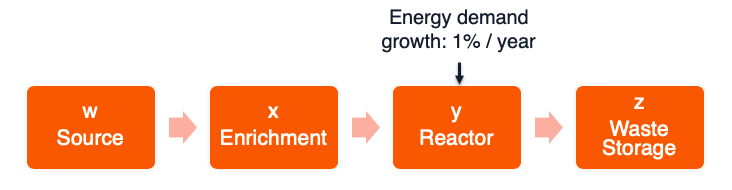
\includegraphics[width=0.8\textwidth]{images/auto-deploy}
      \end{center}
            \caption{Demand Driven Deployment Scheme}
    \end{figure}

  \end{frame}


\section{Accomplishments}
\subsection{GIS Capability}

\begin{frame}
    \frametitle{Cyclus Simulation of historic U.S. nuclear fuel cycle}
    \textbf{A} \textsc{Cyclus} \textbf{simulation of the U.S. nuclear fuel cycle} was created using historic United States reactor deployment data obtained from the Power Reactor Information System (PRIS) database \cite{peterson_unf_2017}.
    \\

    \textbf{Simulation Assumptions} \\
    Facilities present in the simulation: mine, mill, enrichment plant, fuel fabrication facility, 112 historic commercial reactors in the U.S, dry storage facility and a final waste repository.
    \\

    \textbf{Recipe Reactor Facility Assumptions}
    \begin{itemize}
    \item \textit{Refueling time}: 1 month
    \item \textit{Cycle length}: 18 months
    \item \textit{Single Spent Fuel Recipe}: 33 or 51 GWDt/MTU burnup (depletion calculations done using ORIGEN)
    \item \textit{Assembly size, Core size, Batch size}: dependent on the reactor type
    \item \textit{Power cap, Location}: specific to each reactor from PRIS data
    \end{itemize}
  \end{frame}

  \begin{frame}
    \frametitle{CycMap: Cyclus Simulation of historic U.S. nuclear fuel cycle}
    \begin{figure}[htbp!]
      \begin{center}
        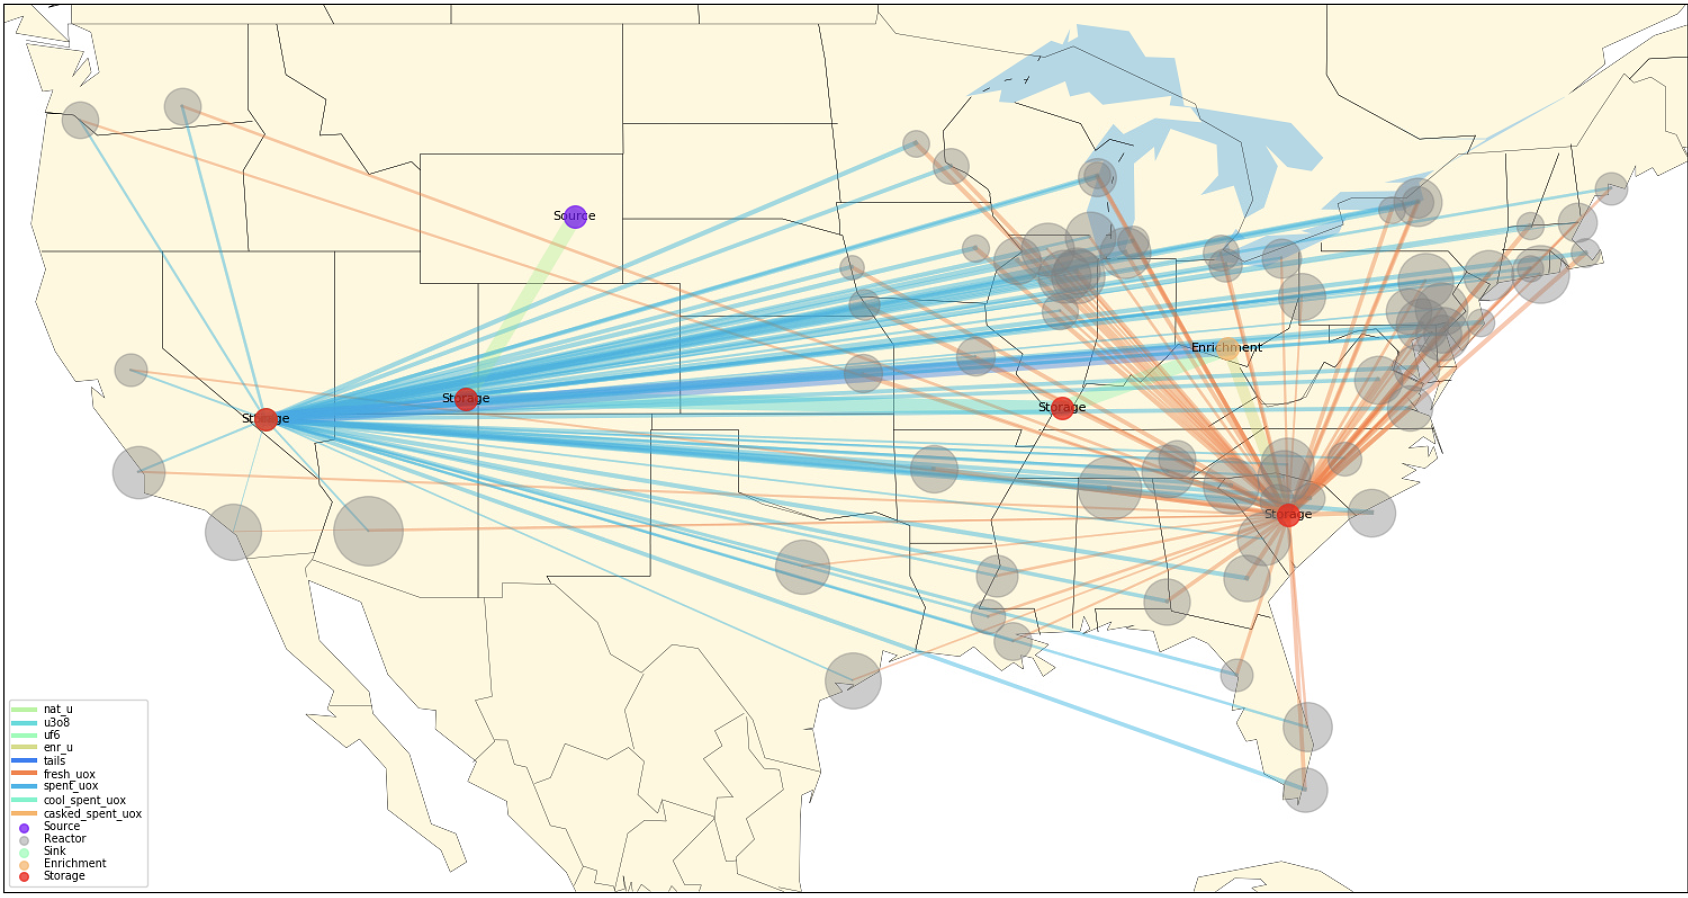
\includegraphics[height=5.5cm]{images/cycmap}
      \end{center}
            \caption{Cycmap of the historic Cyclus U.S nuclear fuel cycle simulation \cite{park_arfc/cycmap_2018}}
    \end{figure}
  \end{frame}

\begin{frame}
  \frametitle{Power demand: Cyclus Simulation of historic U.S. nuclear fuel cycle}
  \begin{columns}
    \column[t]{5cm}
    \begin{figure}[htbp!]
      \begin{center}
        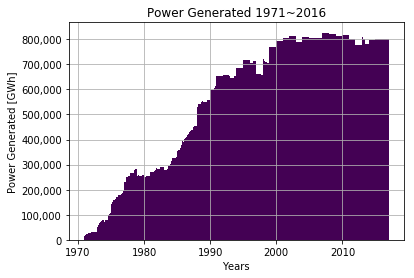
\includegraphics[height=3.5cm]{images/power_gen_cyclus}
      \end{center}
            \caption{Power generated between 1971 and 2016 from the \textsc{Cyclus} simulation}
    \end{figure}
    \column[t]{5cm}
    \begin{figure}[htbp!]
      \begin{center}
        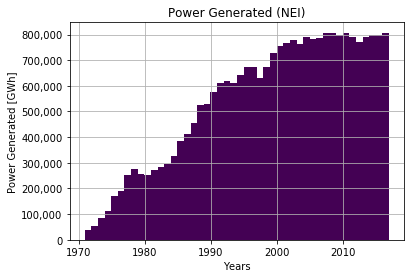
\includegraphics[height=3.5cm]{images/power_gen_nei}
      \end{center}
            \caption{Power generated between 1971 and 2016 as published by the NEI \cite{nei_u.s._2018}}
    \end{figure}
  \end{columns}
\end{frame}

\subsection{Challenge Problem}
\begin{frame}
        \frametitle{Synergistic Spent Nuclear Fuel Dynamics Within the European 
        Union}
\begin{itemize}
       \item Collaborative spent fuel management is materially feasible among nuclear
               nations in the  European Union.
       \item Collaborative EU spent fuel management could expedite a fast reactor
               technology transition in France.
       \item By using spent fuel from other EU nations, France can avoid
               building new light water reactors to support a transition to
               fast reactors.
\end{itemize}
\end{frame}


\begin{frame}
	\frametitle{Deployment Timeline for French Transition}
	110 SFRs (66 GWe) are deployed by 2076.
	\begin{figure}[htbp!]
	\begin{minipage}[b]{.45\linewidth}
        \begin{center}
                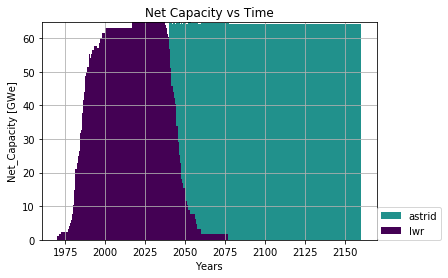
\includegraphics[width=\textwidth]{./images/french-transition/power_plot.png}
        \end{center}
        \caption{French Transition into an SFR Fleet}
        \label{fig:sfr_num}
	\end{minipage}
	\hspace{.5cm}
	\begin{minipage}[b]{.45\linewidth}
		\centering
		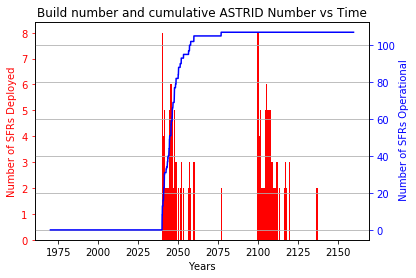
\includegraphics[width=\textwidth]{./images/french-transition/sfr_deploy.png}
		\caption{Deployment of French SFRs and total installed capacity}
		\label{fig:dep}
	\end{minipage}
\end{figure}
\end{frame}



\begin{frame}
\begin{figure}[htbp!]
    \begin{center}
        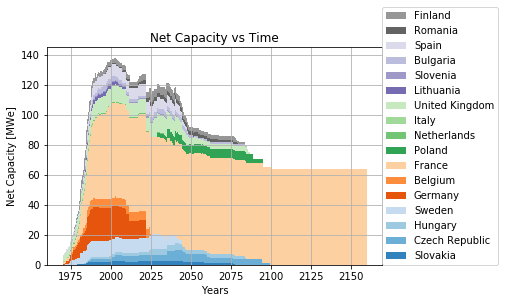
\includegraphics[width=\textwidth]{./images/onesim.png}
    \end{center}
    \caption{The simulated nuclear power deployment scheme relies on used
        nuclear fuel collaboration among nations.
        The historical operation of EU reactors is followed by the French transition to SFRs.  The steep transition from 2040 to 2060 reflects the scheduled decommissioning of reactors built in the 1975-2000 era of aggressive nuclear growth in France.}
    \label{fig:tot_dep}
\end{figure}
\end{frame}


\subsection{\deploy} 
\begin{frame}
    \frametitle{\deploy Objectives}
    \textbf{\deploy's Main Objective}
    \vspace{0.3em}
    \\
    Minimize the number of time steps of undersupply or under capacity 
    of power.
    \vspace{1em}
    \\
    \textbf{\deploy's Sub-Objectives}
    \begin{itemize}
        \item Minimize the number of time steps of undersupply or under capacity 
        of any commodity.
        \item Minimize excessive oversupply of all commodities  
    \end{itemize} 
\end{frame}

\begin{frame}
    \frametitle{\deploy Input Parameters}
    \begin{table}[]
        \centering
        \caption{\deploy's required and optional input parameters with examples.}
		\label{tab:inputs}
            \footnotesize
			\begin{tabularx}{\textwidth}{l|LL}
			\hline
				& \textbf{Input Parameter}                                                           & \textbf{Examples}                                                                                                          \\ \hline
				\multirow{5}{*}{\textbf{Required}} & Demand driving commodity                                                           & Power, Fuel, Plutonium, etc.                                                                                                                      \\ 
														  & Demand equation                                                                    & P(t) = 10000, sin(t), 10000*t                                                                                                                 \\ \cline{2-3} 
														  & Facilities it controls                                                             & Fuel Fab, LWR reactor, SFR reactor, Waste repository, etc.                                                                                                      \\ \cline{2-3} 
														  & Capacities of the facilities                                                       & 3000 kg, 1000 MW, 50000 kg                                                                                                     \\ \cline{2-3} 
														  & Prediction method                                                                  & \begin{tabular}[c]{@{}l@{}}Power: fast fourier transform\\ Fuel: moving average\\ Spent fuel: moving average\end{tabular} \\ \cline{2-3} 
														  & Deployment driven by & Installed Capacity/Supply                                                                                                                    \\ \hline
				\multirow{4}{*}{\textbf{Optional}} & Supply/Capacity Buffer type                                                                        & Absolute                                                                                                                  \\ \cline{2-3} 
														  & Supply/Capacity Buffer size                                                                        & \begin{tabular}[c]{@{}l@{}}Power: 3000 MW\\ Fuel: 0 kg \\ Spent fuel: 0 kg\end{tabular}                                   \\ \cline{2-3} 
														  & Facility preferences                                                               & \begin{tabular}[c]{@{}l@{}}LWR reactor = 100-t\\ SFR reactor = t-100 \end{tabular}          \\ \cline{2-3} 
														  & Facility constraint                                                              & SFR reactor constraint = 5000kg of Pu            \\ \hline	
						\end{tabularx}
    \end{table}
\end{frame}

\begin{frame}
    \frametitle{\deploy logic flow}
    \begin{columns}
        \column[t]{8cm}
    \begin{figure}[]
        \centering
        \resizebox{0.8\textwidth} {0.5\height}{
        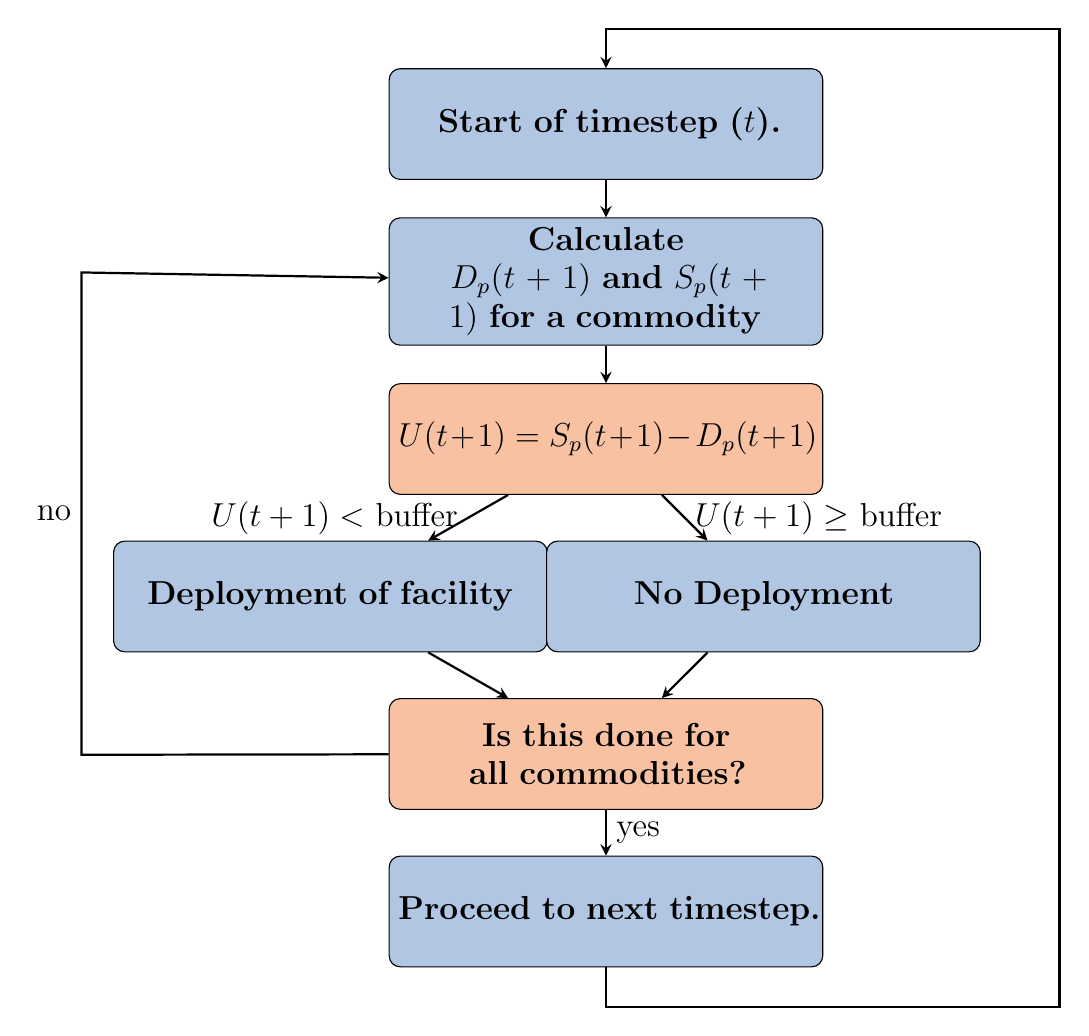
\begin{tikzpicture}[node distance=2cm]
        \tikzstyle{every node}=[font=\large]
        \node (Start) [bblock] {\textbf{Start of timestep ($t$).}};
        \node (Predict) [bblock, below of=Start] {\textbf{Calculate \\ $D_p(t+1)$ and $S_p(t+1)$ for a commodity}};
        \node (IsThere) [oblock, below of=Predict]{\textbf{$U(t+1) = S_p(t+1)-D_p(t+1)$}};
        \node (Deploy) [bblock, below of=IsThere, xshift = -3.5cm]{\textbf{Deployment of facility}};
        \node (NoDeploy) [bblock, right of=Deploy, xshift = 3.5cm]{\textbf{No Deployment} };
        \node (All) [oblock, below of=Deploy, xshift = 3.5cm] {\textbf{Is this done for all commodities?}};
        \node (End) [bblock, below of=All] {\textbf{Proceed to next timestep.}};
        
        \draw [arrow] (Start) -- (Predict); 
        \draw [arrow] (Predict) -- (IsThere);
        \draw [arrow] (IsThere) -- node[anchor=east] {$U(t+1) <$ buffer} (Deploy);
        \draw [arrow] (IsThere) -- node[anchor=west] {$U(t+1) \geq$ buffer} (NoDeploy);
        \draw [arrow] (Deploy) -- (All);
        \draw [arrow] (NoDeploy) -- (All);
        \draw [arrow] (All) -- node[anchor=west] {yes} (End);
        \draw [arrow] (All) -- ([shift={(-3.9cm,0.7cm)}]All.south west)-- node[anchor=east] {no} ([shift={(-3.9cm,-0.7cm)}]Predict.north west)--(Predict);
        \draw [arrow] (End) |-([shift={(3cm,-0.5cm)}]End.south east)-- ([shift={(3cm,0.5cm)}]Start.north east)-|(Start);
        \end{tikzpicture}
        }
        \caption{\deploy logic flow at every timestep in \Cyclus \cite{chee_demonstration_2019}.}
        \label{fig:flow}
    \end{figure}
    \column[t]{5cm}
    \vspace{2cm}
    \\
    $D_p : Predicted Demand$ \\
    $S_p : Predicted Supply$ \\
    $U = S_p-D_p$
\end{columns}
\end{frame}

\begin{frame}
    \frametitle{\deploy Prediction Methods}
    Non-Optimizing Methods 
    \begin{itemize}
        \item Moving Average (\texttt{ma})
        \item Autoregressive Moving Average (\texttt{arma})
        \item Autoregressive Heteroskedasticity (\texttt{arch})
    \end{itemize}
    Deterministic-Optimizing Methods 
    \begin{itemize}
        \item Fast Fourier Transform (\texttt{fft})
        \item Polynomial Fit (\texttt{poly})
        \item Exponential Smoothing
        \item Triple Exponential Smoothing (\texttt{holt-winters})
    \end{itemize}
    Stochastic-Optimizing Methods 
    \begin{itemize}
        \item Auto-Regressive Integrated Moving Averages (\texttt{ARIMA})
    \end{itemize}
\end{frame}
\begin{frame}
    \frametitle{Breakdown of Results}
    4 transition scenarios sought to minimize undersupply and under capacity of 
        all commodities.
    \begin{enumerate}
            \item EG01-23 ($P(t) = P_0$)
        \item EG01-24 ($P(t) = P_0 + rt$)
        \item EG01-29 ($P(t) = P_0)$
        \item EG01-30 ($P(t) = P_0 + rt$)
    \end{enumerate}

This is achieved by:
\begin{enumerate}
    \item Comparison of prediction methods for each of 4 scenarios is conducted 
    to determine the best method. 
    \item Sensitivity analysis of power supply buffer is conducted to determine 
    best buffer size. 
    \item Using best prediction method, look ahead rate, buffer size, demonstrate \deploy 
    deploying reactor and supporting facilities to meet power demand 
    for 4 scenarios. 
\end{enumerate}

\end{frame}


\begin{frame}
        \frametitle{EG01 - EG23}

\begin{figure}[H]
	\centering
	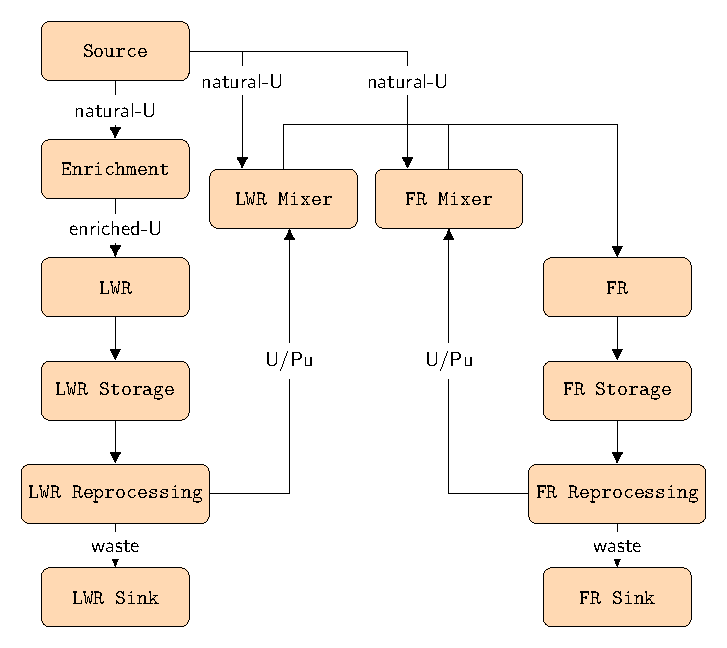
\includegraphics[width=\textwidth]{images/23flow.pdf}
	\hfill
	\caption{EG01-EG23 fuel cycle as modeled in \cyclus.}
	\label{fig:23flow}
\end{figure}
\end{frame}





\begin{frame}
        \frametitle{EG01 - EG23}

\begin{figure}[H]
	\centering
	\includegraphics[width=\textwidth]{images/30flow.pdf}
	\hfill
	\caption{EG01-EG30.}
	\label{fig:30flow}
\end{figure}


\subsection{Comparison of Prediction Methods}
\begin{frame}
    \frametitle{Comparison of Prediction Methods}
\textbf{EG01-23 Constant Power Demand Transition Scenario}

\begin{figure}[htbp!]
    \begin{center}
      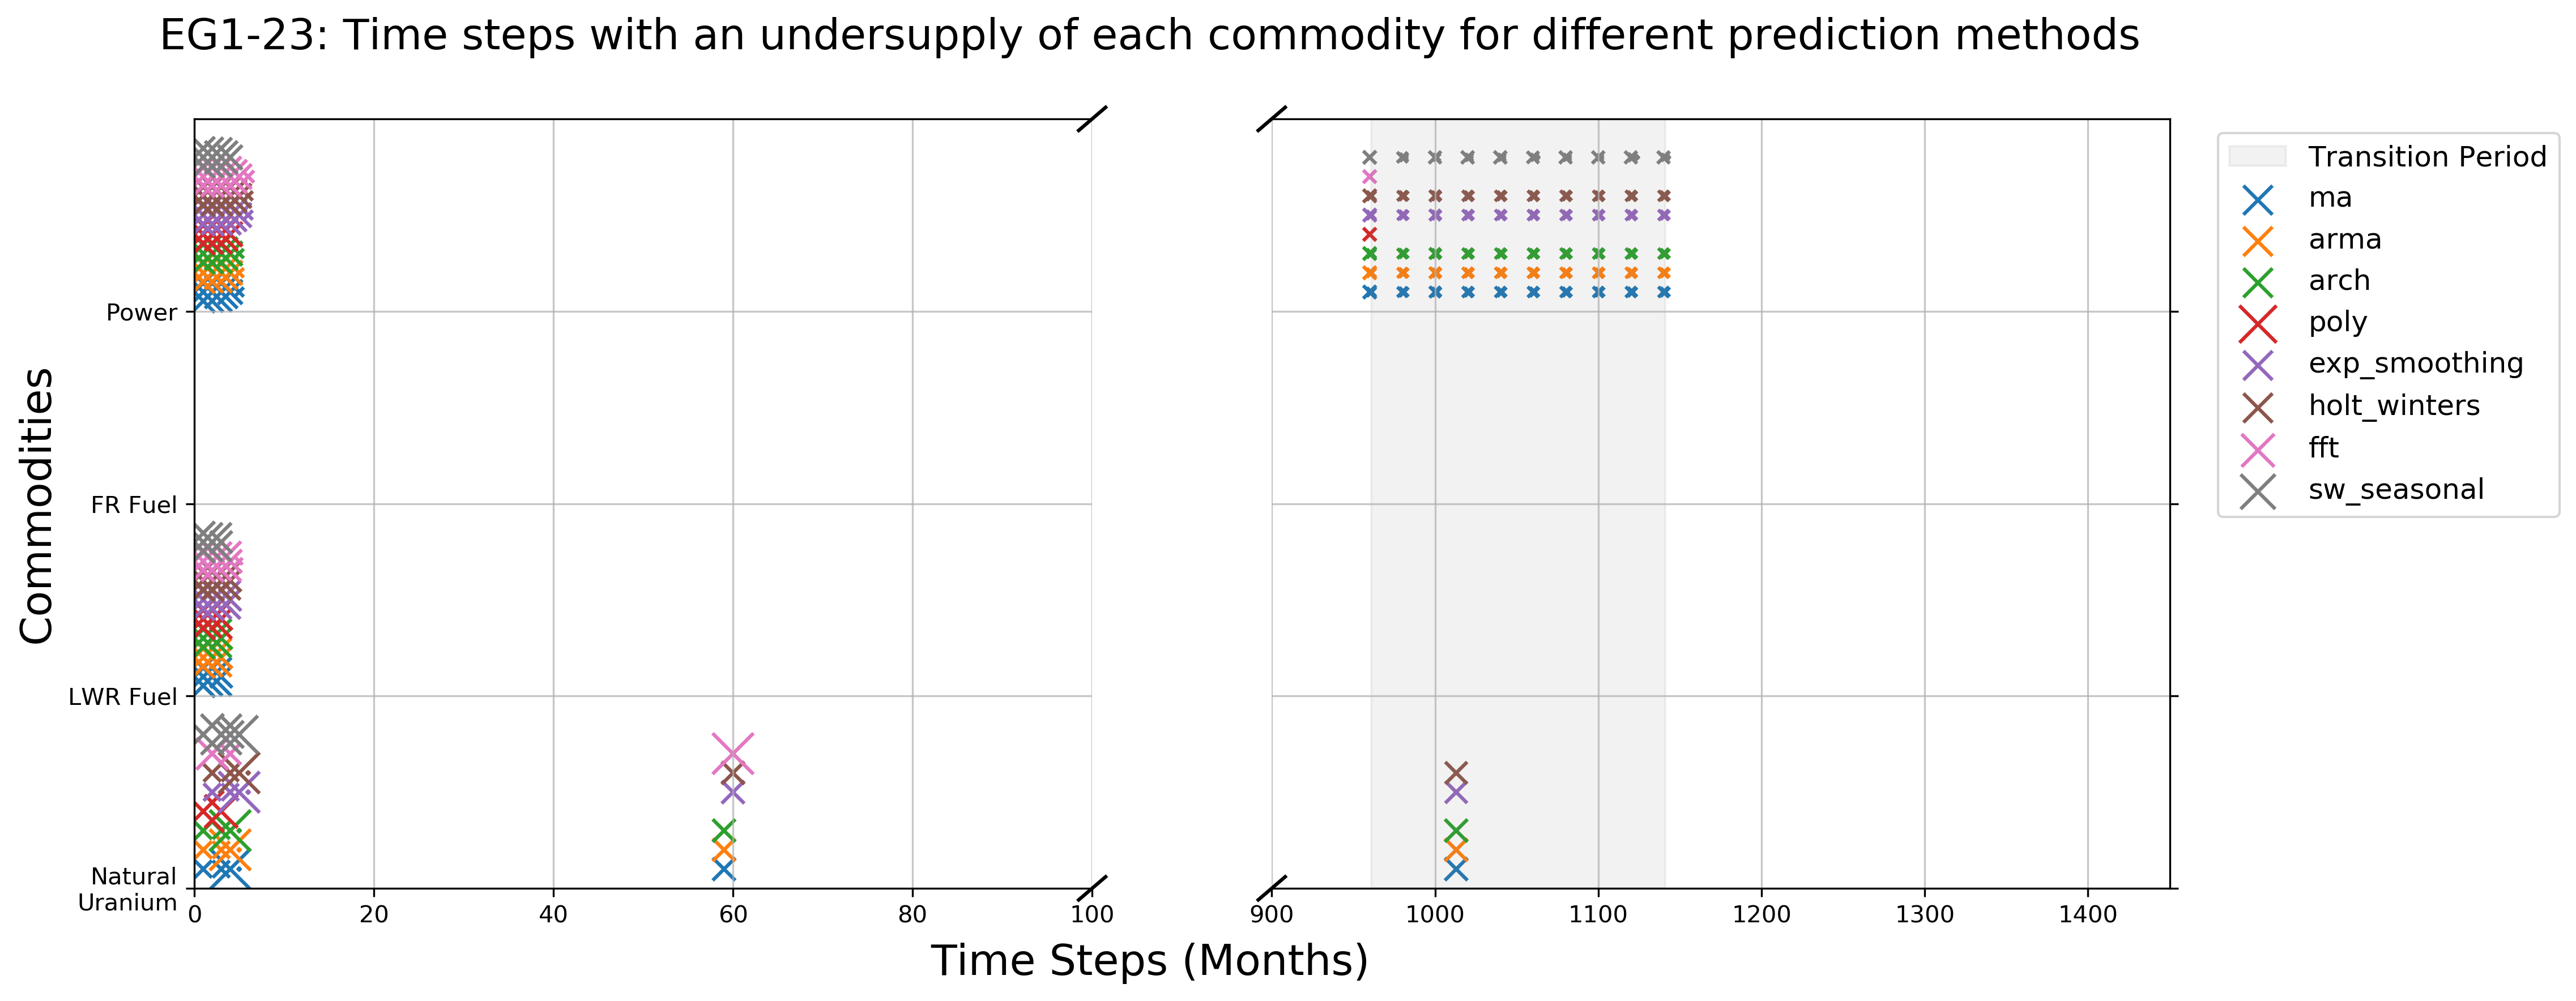
\includegraphics[width=\textwidth]{../paper/figures/eg23-undersupply.png}
    \end{center}
          \caption{Time dependent undersupply of commodities for different
          prediction methods for the EG01-23 Transition Scenario with Constant Power Demand. The
          size of each cross is based on the size of the undersupply.
          Fewer crosses on plot indicates the method is more successful at preventing undersupply 
          of each commodity}
  \end{figure}
\end{frame}

\begin{frame}
    \frametitle{Comparison of Prediction Methods}
    \textbf{EG01-23 Constant Power Demand Transition Scenario}
\begin{figure}[htbp!]
    \begin{center}
      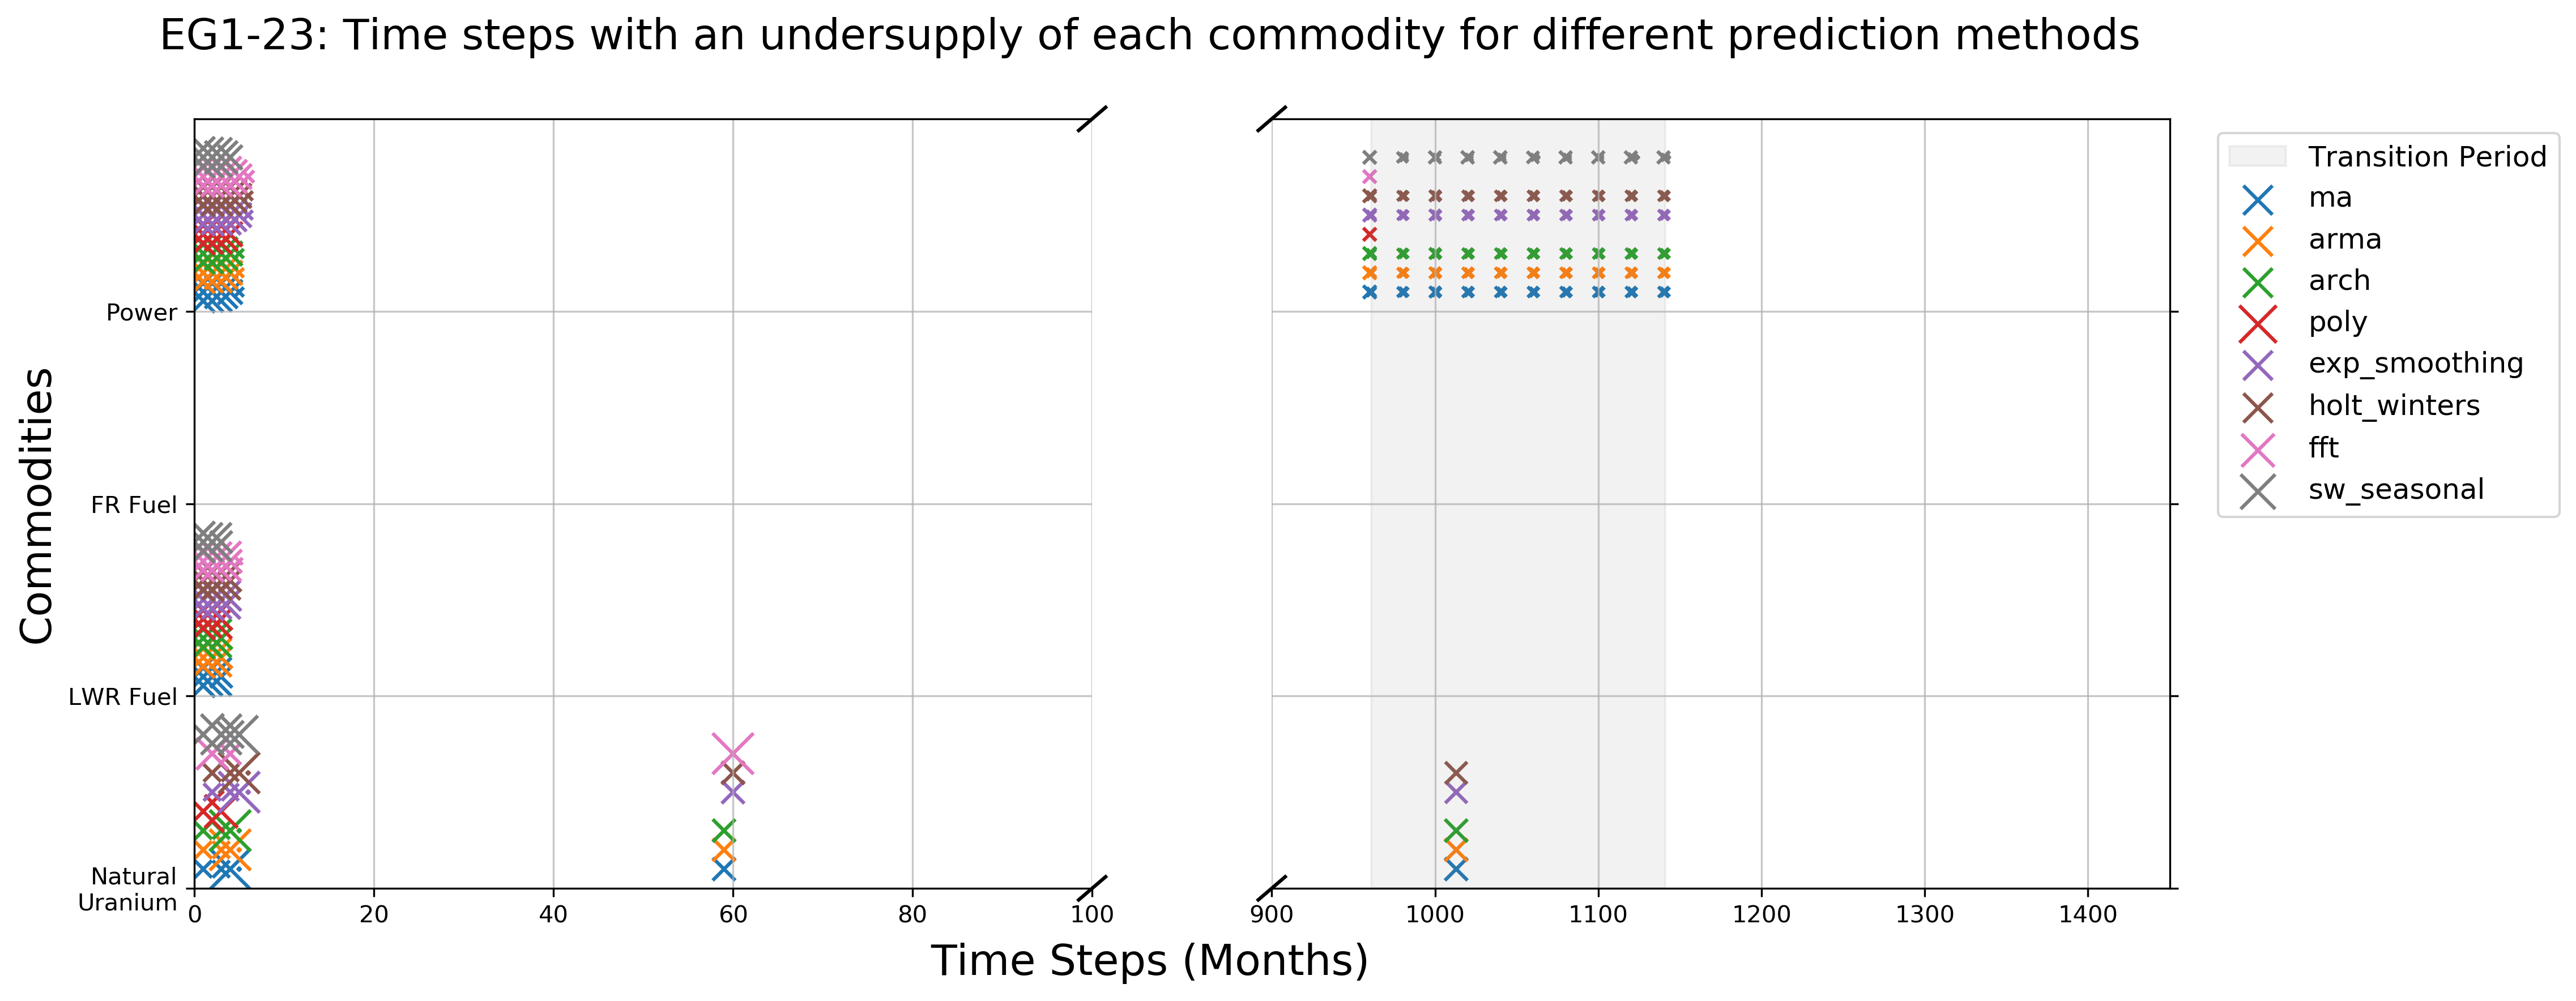
\includegraphics[width=\textwidth]{../paper/figures/eg23-undersupply.png}
    \end{center}
          \caption{Time dependent undersupply of commodities for different
          prediction methods for the EG01-23 Transition Scenario with Constant Power Demand. The
          size of each cross is based on the size of the undersupply.
          Fewer crosses on plot indicates the method is more successful at preventing under capacity 
          of each commodity}
  \end{figure}
\end{frame}

\begin{frame}
    \frametitle{Comparison of Prediction Methods}
\textbf{EG01-24 Constant Power Demand Transition Scenario}
\begin{figure}[htbp!]
    \begin{center}
      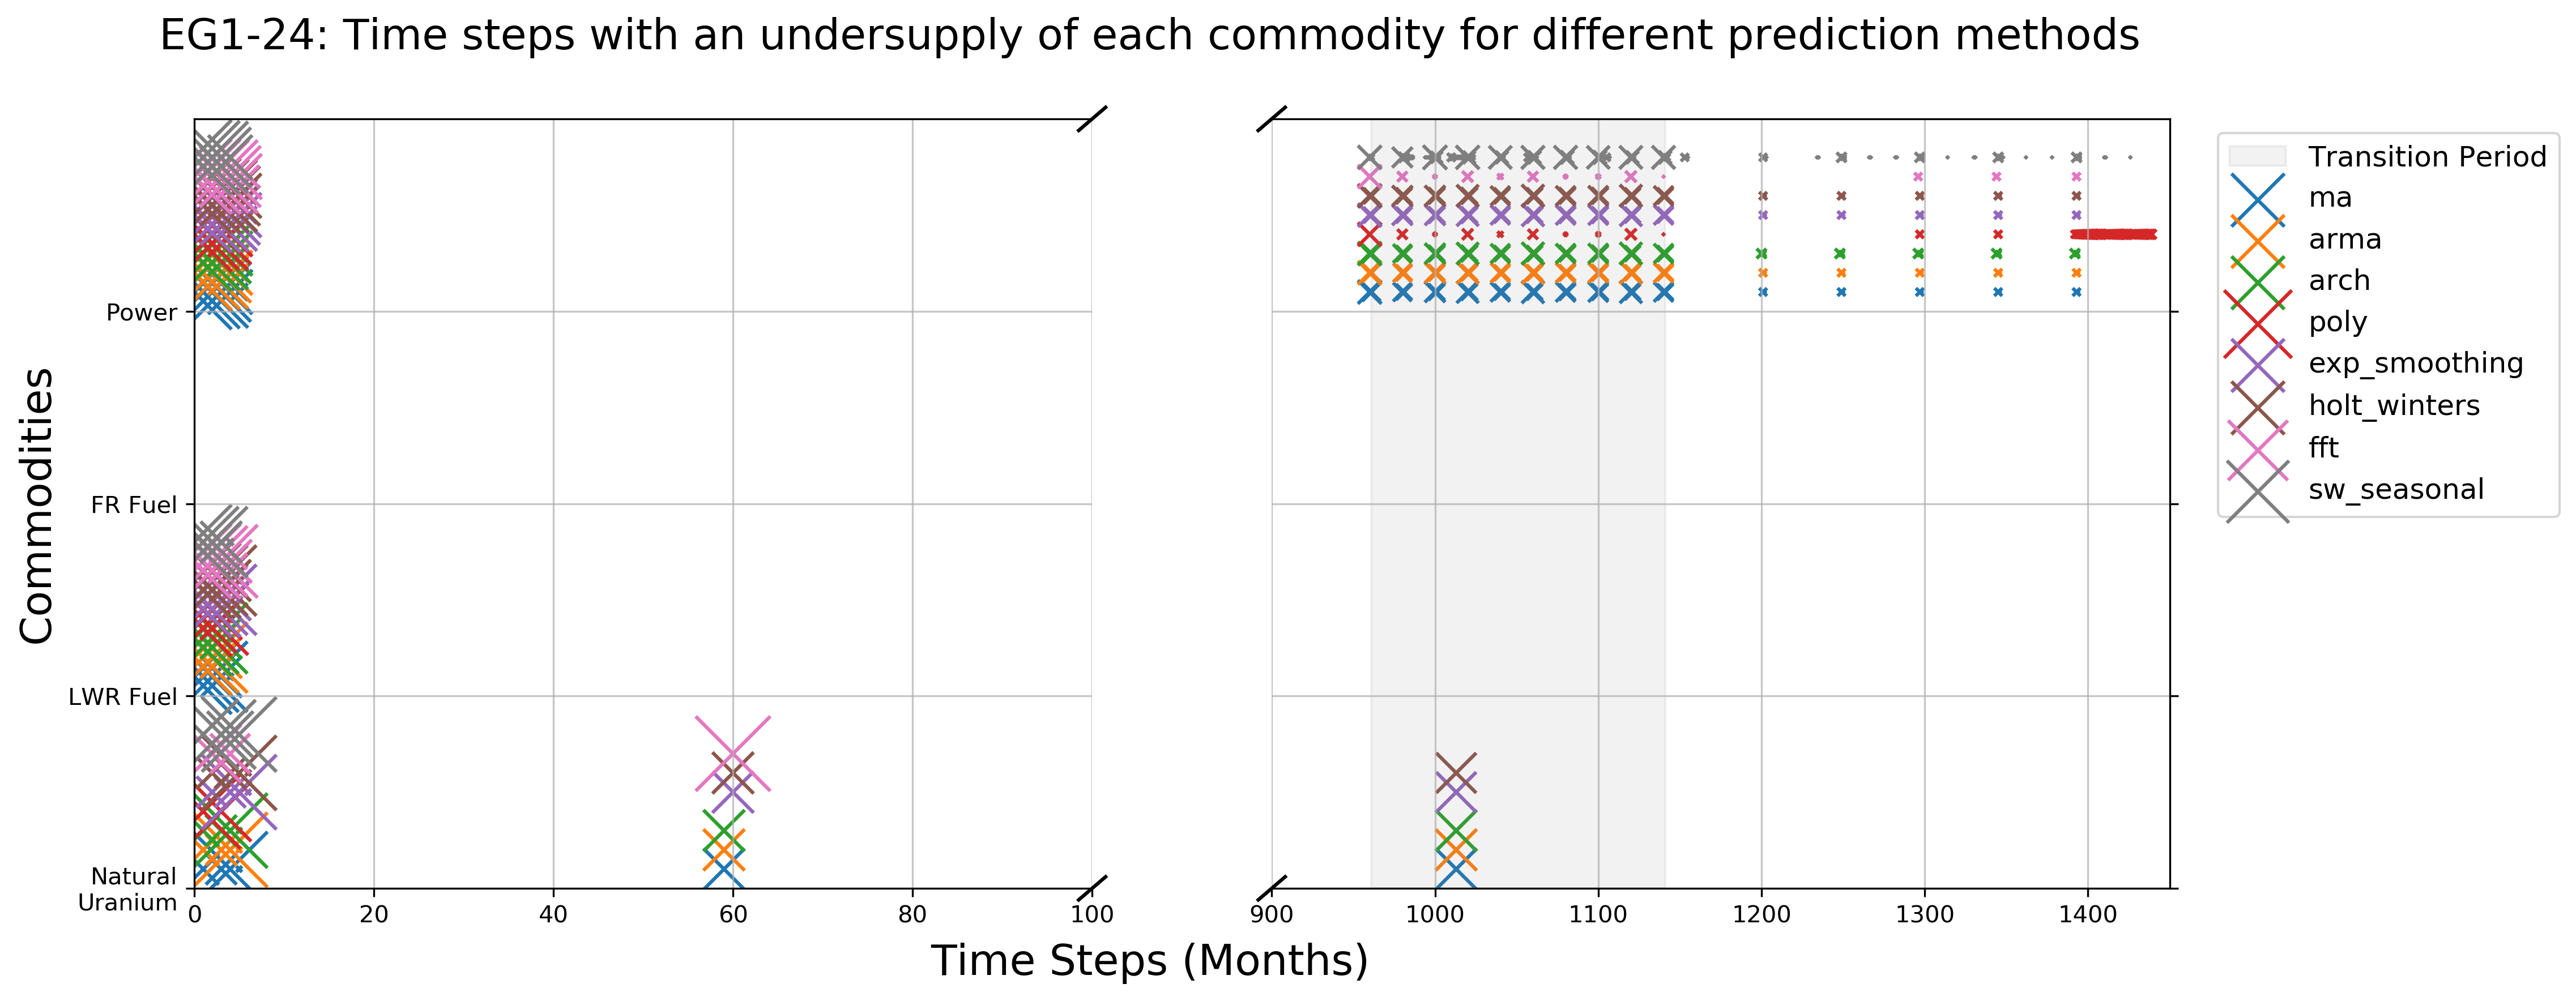
\includegraphics[width=\textwidth]{../paper/figures/eg24-undersupply.png}
    \end{center}
          \caption{Time dependent undersupply of commodities for different
          prediction methods for the EG01-24 Transition Scenario with Linearly Increasing Power Demand.The
          size of each cross is based on the size of the undersupply.
          Fewer crosses on plot indicates the method is more successful at preventing undersupply 
          of each commodity}
  \end{figure}
\end{frame}

\begin{frame}
    \frametitle{Comparison of Prediction Methods}
    \textbf{EG01-24 Constant Power Demand Transition Scenario}
\begin{figure}[htbp!]
    \begin{center}
      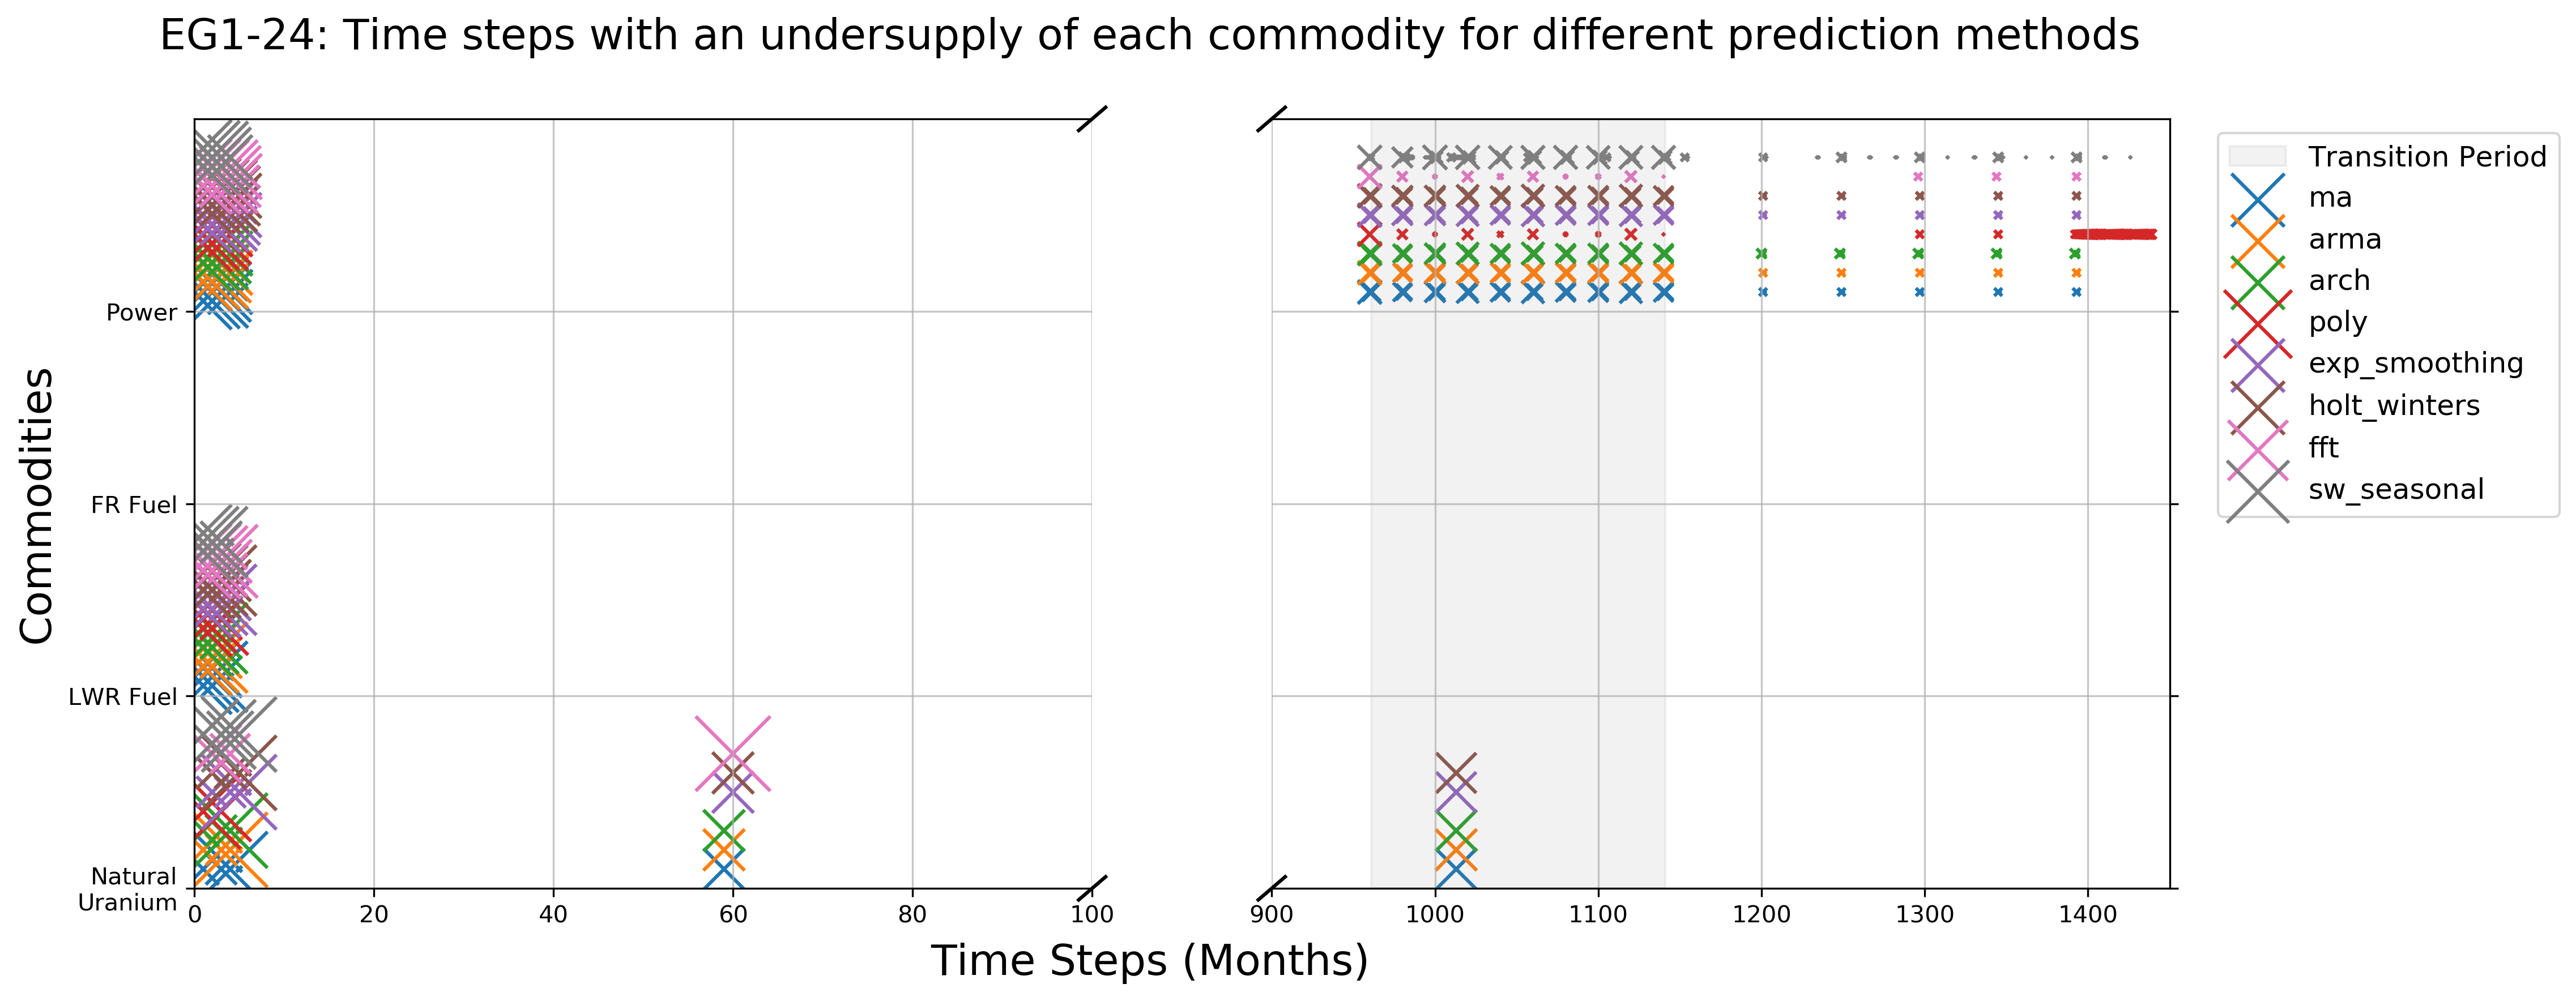
\includegraphics[width=\textwidth]{../paper/figures/eg24-undersupply.png}
    \end{center}
          \caption{Time dependent undersupply of commodities for different
          prediction methods for the EG01-24 Transition Scenario with Linearly Increasing Power Demand. The
          size of each cross is based on the size of the under capacity.
          Fewer crosses on plot indicates the method is more successful at preventing under capacity
          of each commodity}
  \end{figure}
\end{frame}

\begin{frame}
  \frametitle{Comparison of Prediction Methods}
  \textbf{Main Takeaway}
  \\
  The best performing prediction method for each transition scenario is: 
  \begin{enumerate}
    \item EG01-23 Constant Power Demand: \texttt{poly}
    \item EG01-24 Linearly Increasing Power Demand: \texttt{fft}
    \item EG01-29 Constant Power Demand: \texttt{poly}
    \item EG01-30 Linearly Increasing Power Demand: \texttt{fft}
\end{enumerate}
\end{frame}
\begin{frame}
    \frametitle{Sensitivity Analysis of Power Buffer}
    \textbf{EG01-24}: Linearly Increasing Power Demand
    \begin{figure}[htbp!]
        \begin{center}
          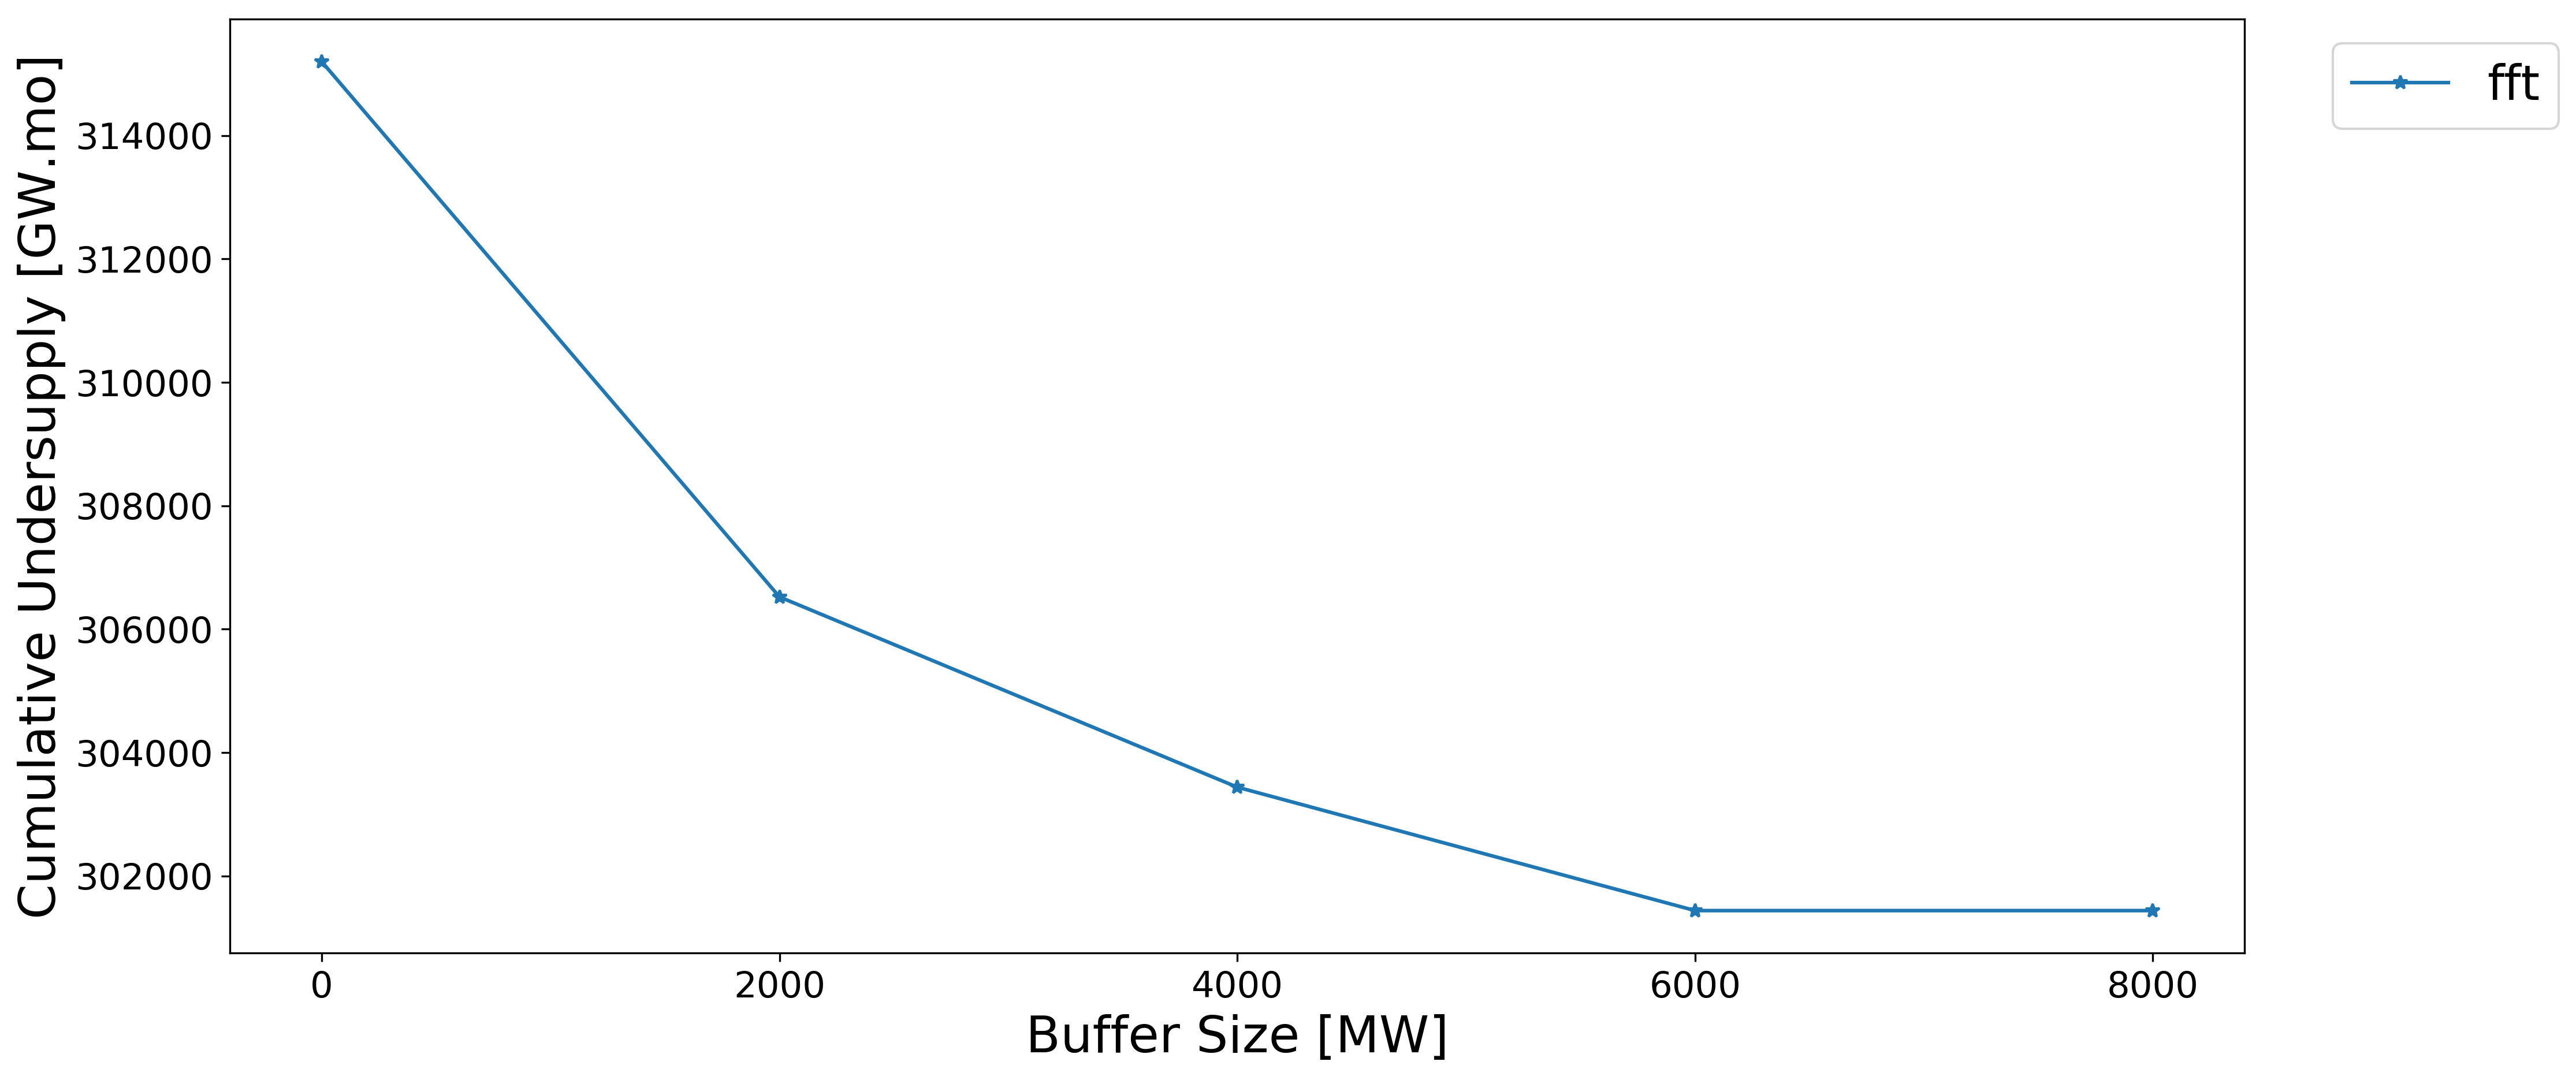
\includegraphics[width=0.8\textwidth]{images/24-sens-buffer}
        \end{center}
              \caption{Sensitivity Analysis of Power buffer size on cumulative 
              undersupply of Power for EG01-EG24 transition scenarios 
              with linearly increasing power demand using the fft prediction method.}
      \end{figure}
\end{frame}

\begin{frame}
    \frametitle{Sensitivity Analysis of Power Buffer}
    \textbf{EG01-30}: Linearly Increasing Power Demand
    \begin{figure}[htbp!]
        \begin{center}
          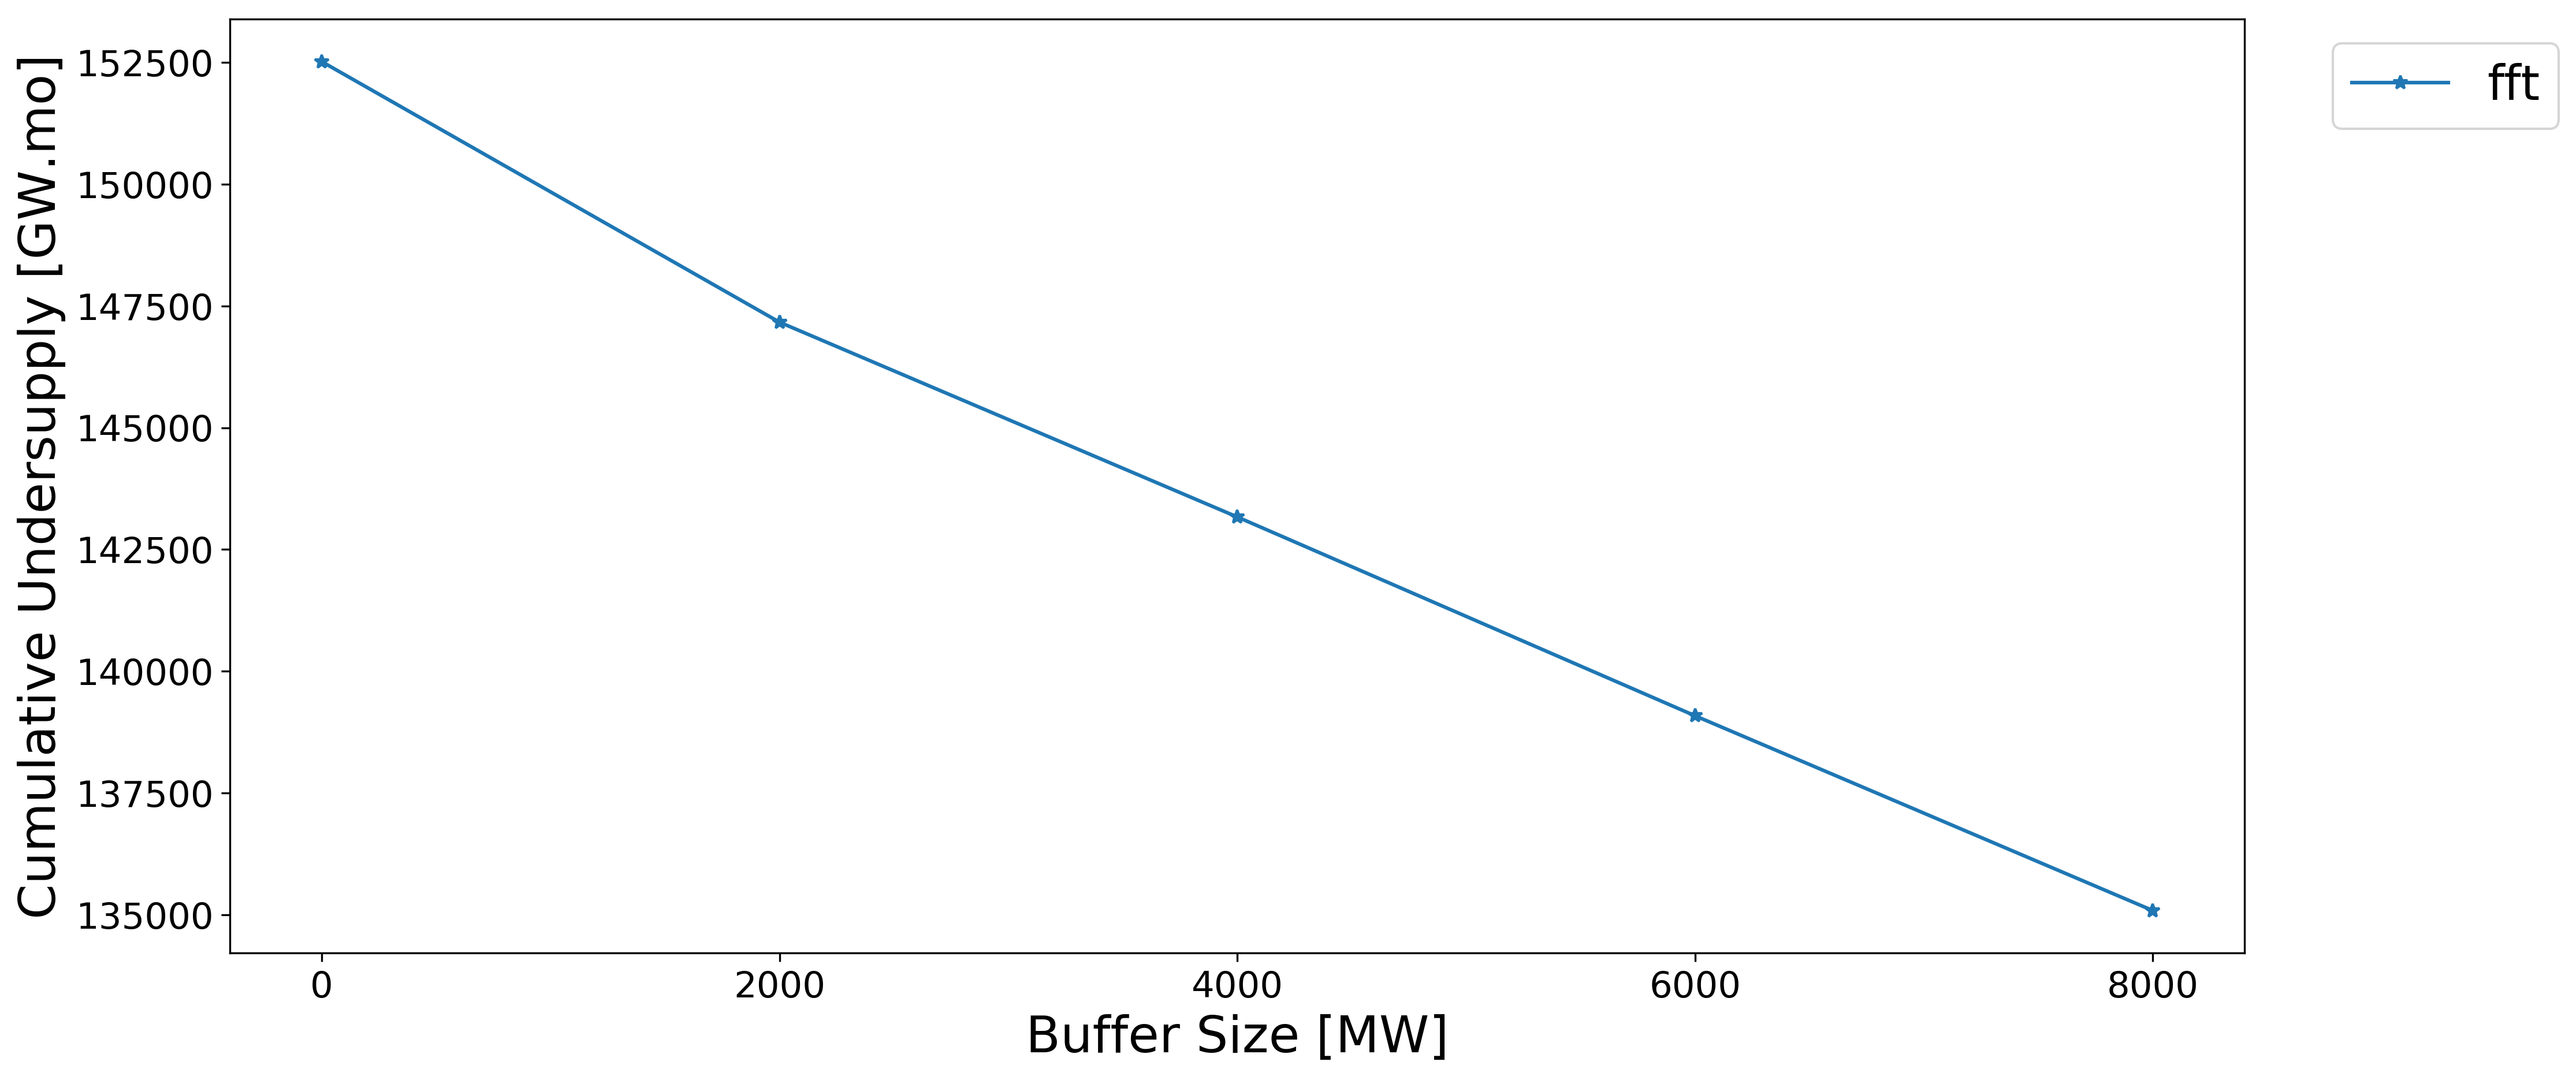
\includegraphics[width=0.8\textwidth]{images/30-sens-buffer}
        \end{center}
              \caption{Sensitivity Analysis of Power buffer size on cumulative 
              undersupply of Power for EG01-EG30 transition scenarios 
              with linearly increasing power demand using the fft prediction method.}
      \end{figure}
\end{frame}

\begin{frame}
  \frametitle{Sensitivity Analysis of Power Buffer}
  \textbf{Main Takeaway}
  \\
  The best power supply buffer for each transition scenario is: 
  \begin{enumerate}
    \item EG01-23 Constant Power Demand: 0 MW
    \item EG01-24 Linearly Increasing Power Demand: 6000 MW
    \item EG01-29 Constant Power Demand: 0 MW
    \item EG01-30 Linearly Increasing Power Demand: 8000 MW 
\end{enumerate}
\end{frame}

\begin{frame}
    \frametitle{Best Performing Transition Scenarios}
    \textbf{Input Parameters of best performing transition scenarios}
    \begin{table}[]
        \resizebox{\textwidth}{!}{%
        \begin{tabular}{|l|l|c|l|l|l|}
        \hline
        \multirow{2}{*}{}                         & \multicolumn{1}{c|}{\multirow{2}{*}{\textbf{Input Parameter}}} & \multicolumn{4}{c|}{\textbf{Simulation Description}}                                                                                                                                                                                                                                                       \\ \cline{3-6} 
                                                  & \multicolumn{1}{c|}{}                                          & \multicolumn{1}{l|}{\textbf{EG01-23}}                                                                 & \textbf{EG01-24}                  & \textbf{EG01-29}                 &\textbf{EG01-30}                                                  \\ \hline
        \multirow{4}{*}{\textbf{Required}} & Demand driving commodity                                       & \multicolumn{4}{c|}{Power}                                                                                                                                                                                                                                                                                 \\ \cline{2-6} 
                                                  & Demand equation [MW]                                               & \multicolumn{1}{l|}{60000}                                                                                & $60000 + 250t/12$ & 60000                     &     $60000 + 250t/12$                                       \\ \cline{2-6} 
                                                  & Prediction method                                              & \texttt{poly}       & \texttt{fft}             & \texttt{poly}         &  \texttt{fft}    \\ \cline{2-6} 
                                                  & Deployment Driving Method                                      & \multicolumn{4}{c|}{Installed Capacity}                                                                                                                                                                                                                                                                    \\ \hline
        \multirow{2}{*}{\textbf{Optional}} & Buffer type                                                    & \multicolumn{4}{c|}{Absolute}                                                                                                                                                                                                                                                               \\ \cline{2-6} 
                                                  & Power Buffer size [MW]                                                   & 0 & 6000 & 0 & 8000 \\ \hline
        \end{tabular}%
        }
        \caption{\deploy's input parameters for EG01-EG23, EG01-EG24, EG01-EG29, and 
        EG01-EG30 transition scenarios
        that minimizes undersupply of power and minimizes 
        the undersupply and under capacity of the other facilities. }
        \label{tab:bestinputs}
        \end{table}
\end{frame}

\begin{frame}
    \frametitle{Best Performing Transition Scenarios}
    \textbf{EG01-23: Constant Power Demand}
    \begin{figure}[htbp!]
        \begin{center}
          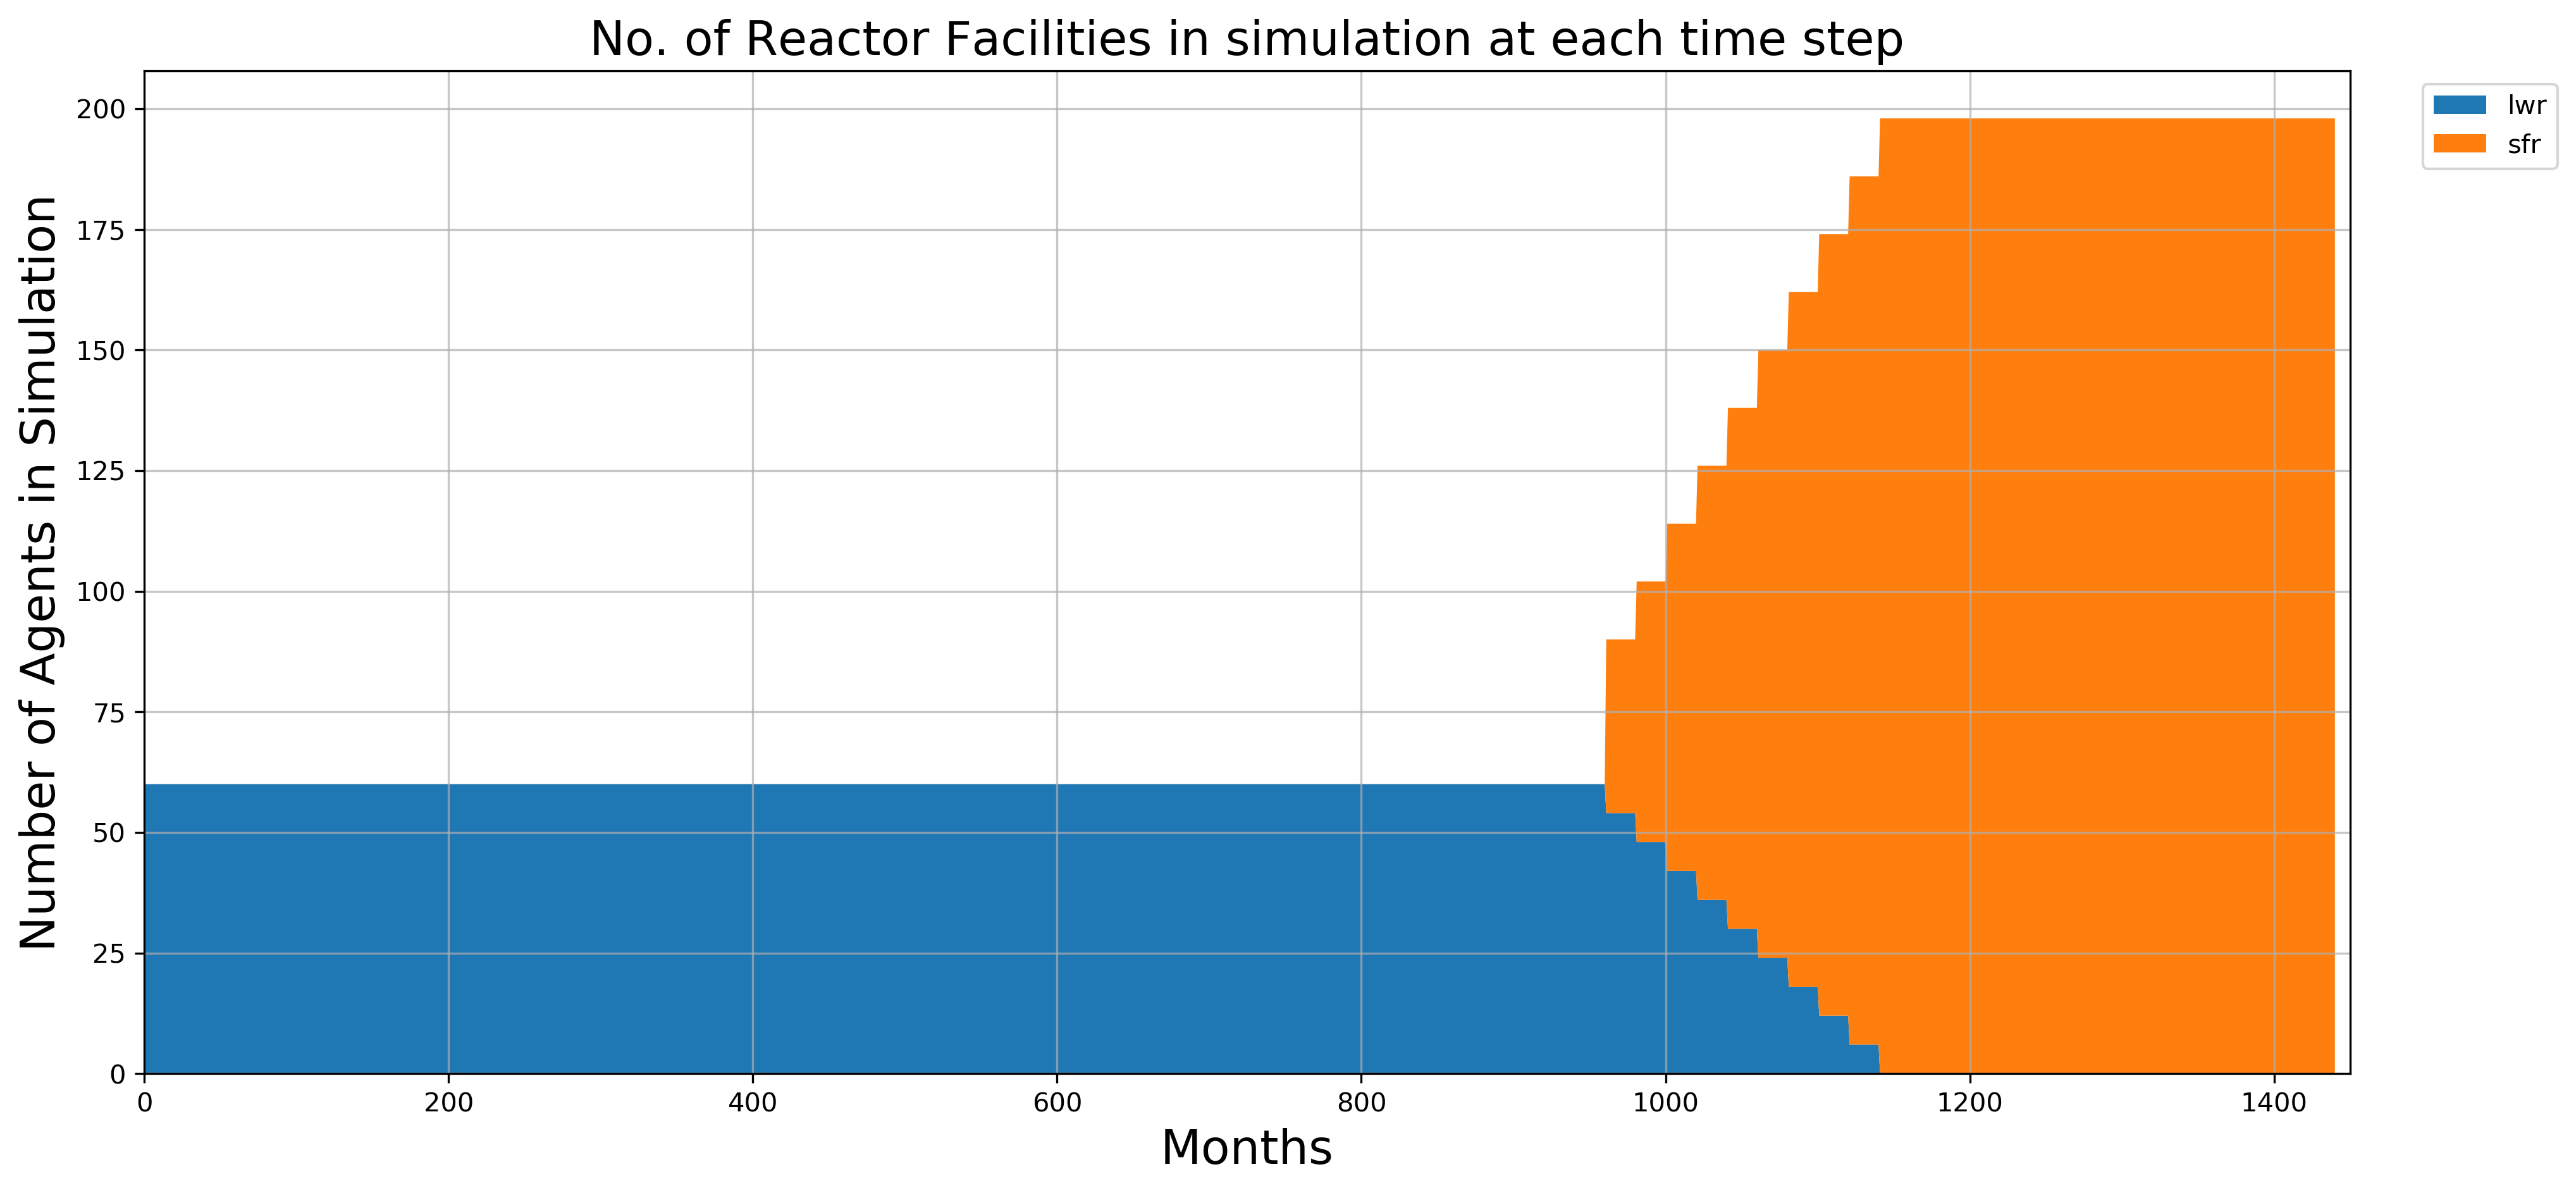
\includegraphics[width=\textwidth]{../paper/figures/eg23-stack_reactor.png}
        \end{center}
              \caption{Time dependent deployment of reactor facilities in 
              the EG01-23 constant power demand transition scenario. 
              \deploy automatically deploys reactor facilities 
              to set up a supply chain to meet constant power demand of $60000$ MW
              during a transition from \glspl{LWR} to \glspl{SFR}}.
      \end{figure}
\end{frame}

\begin{frame}
    \frametitle{Best Performing Transition Scenarios}
    \textbf{EG01-23: Constant Power Demand}
    \begin{figure}[htbp!]
        \begin{center}
          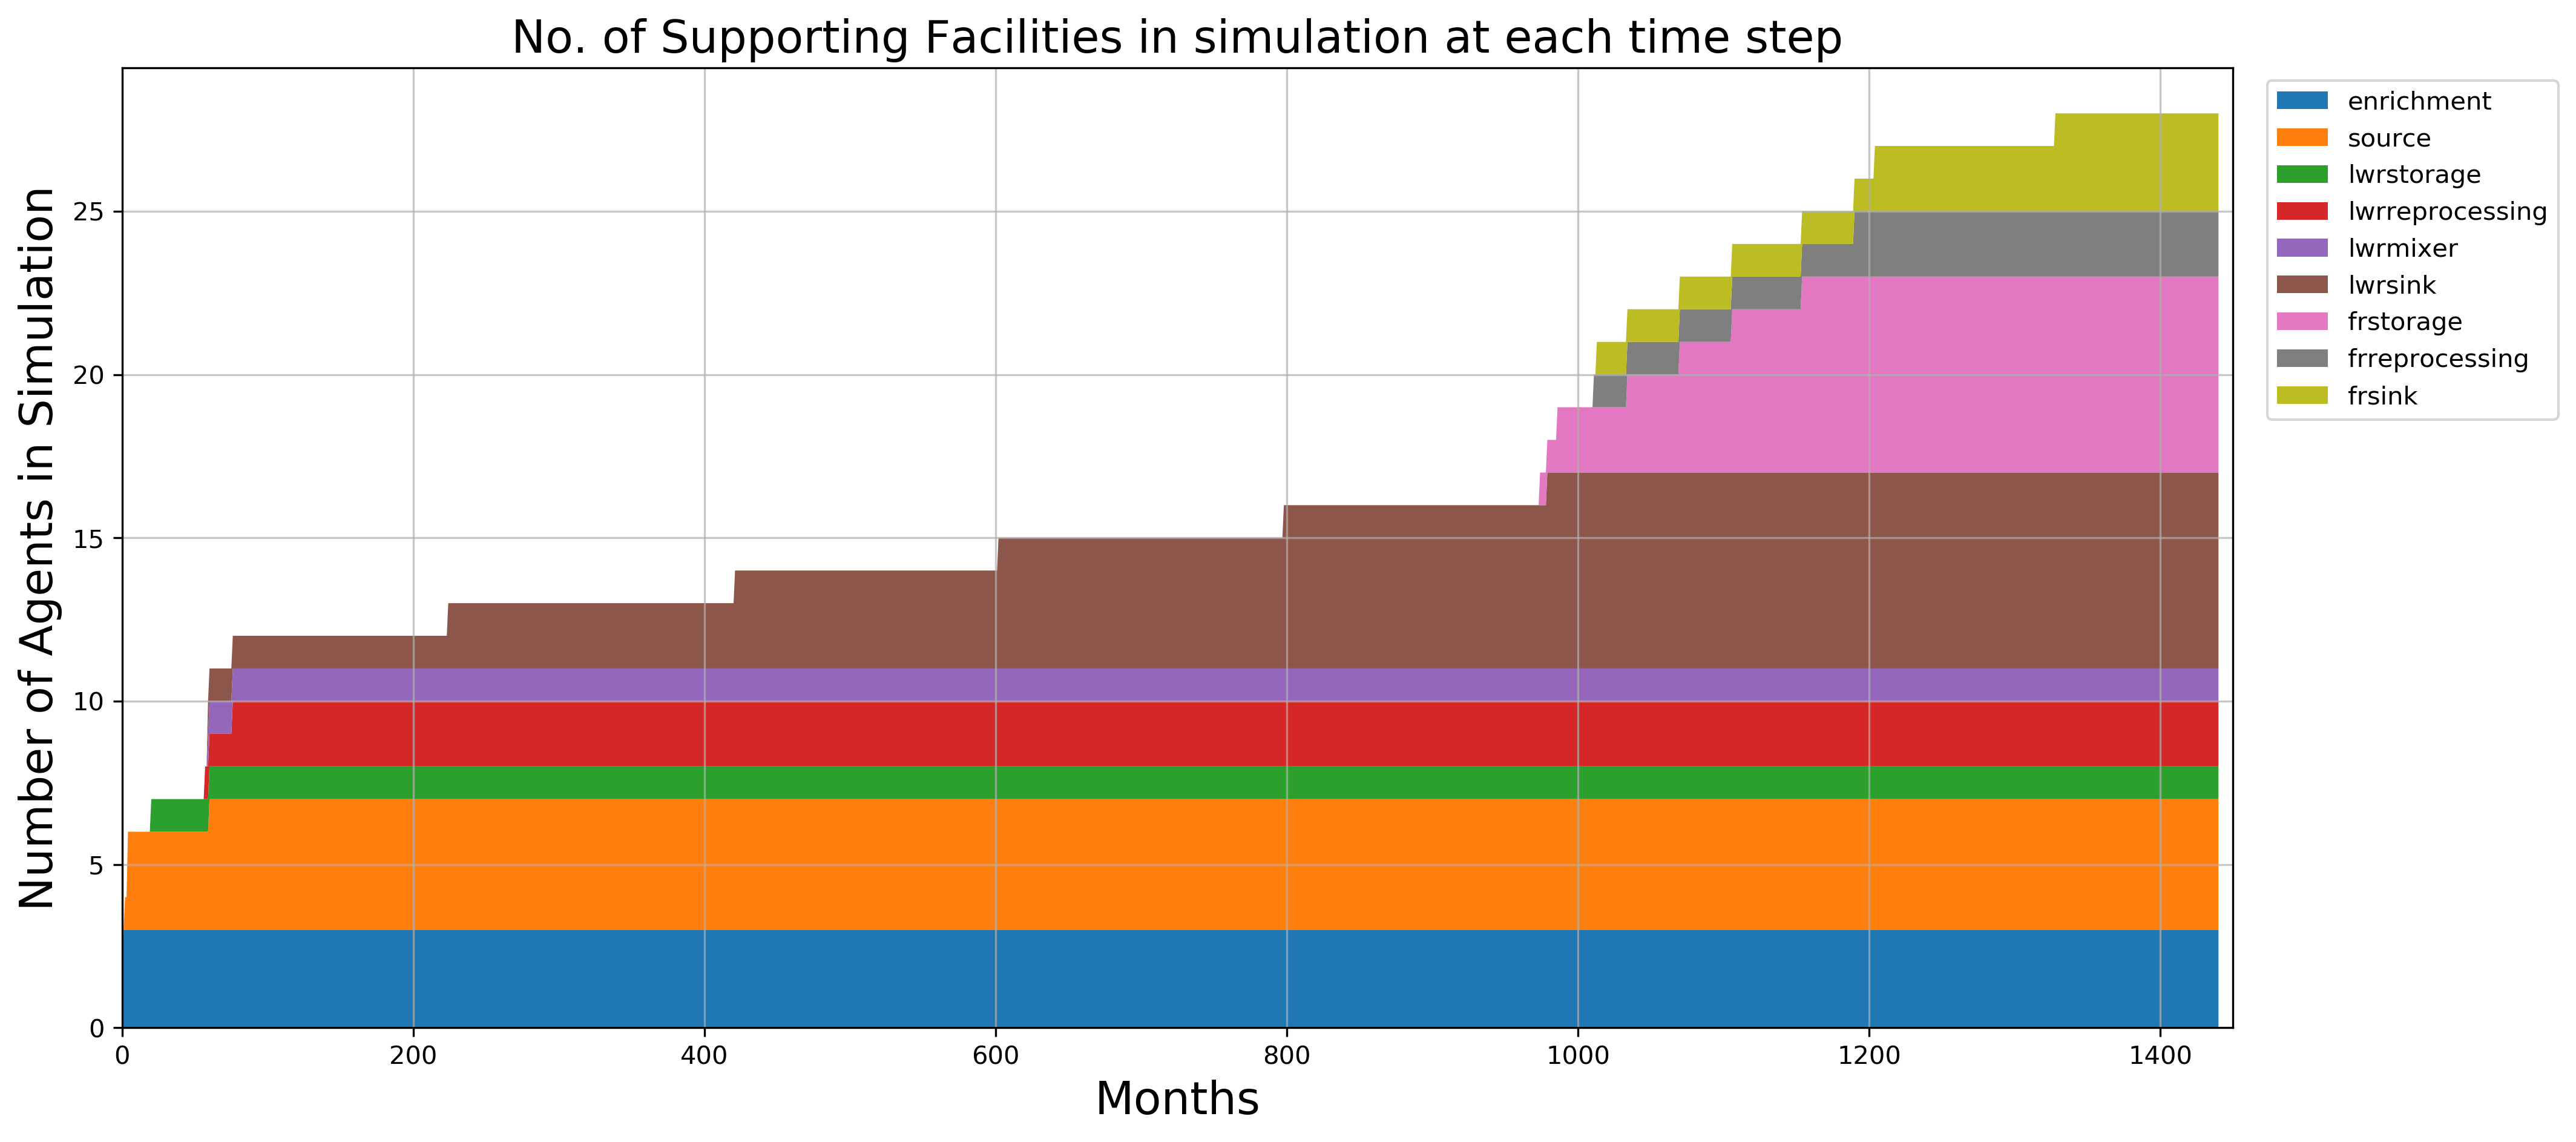
\includegraphics[width=\textwidth]{../paper/figures/eg23-stack_support.png}
        \end{center}
              \caption{Time dependent deployment of supporting facilities in 
              the EG01-23 constant power demand transition scenario. 
              \deploy automatically deploys reactor facilities 
              to set up a supply chain to meet constant power demand of $60000$ MW
              during a transition from \glspl{LWR} to \glspl{SFR}}.
      \end{figure}
\end{frame}

\begin{frame}
    \frametitle{Best Performing Transition Scenarios}
    \textbf{EG01-30: Linearly Increasing Power Demand}
    \begin{figure}[htbp!]
        \begin{center}
          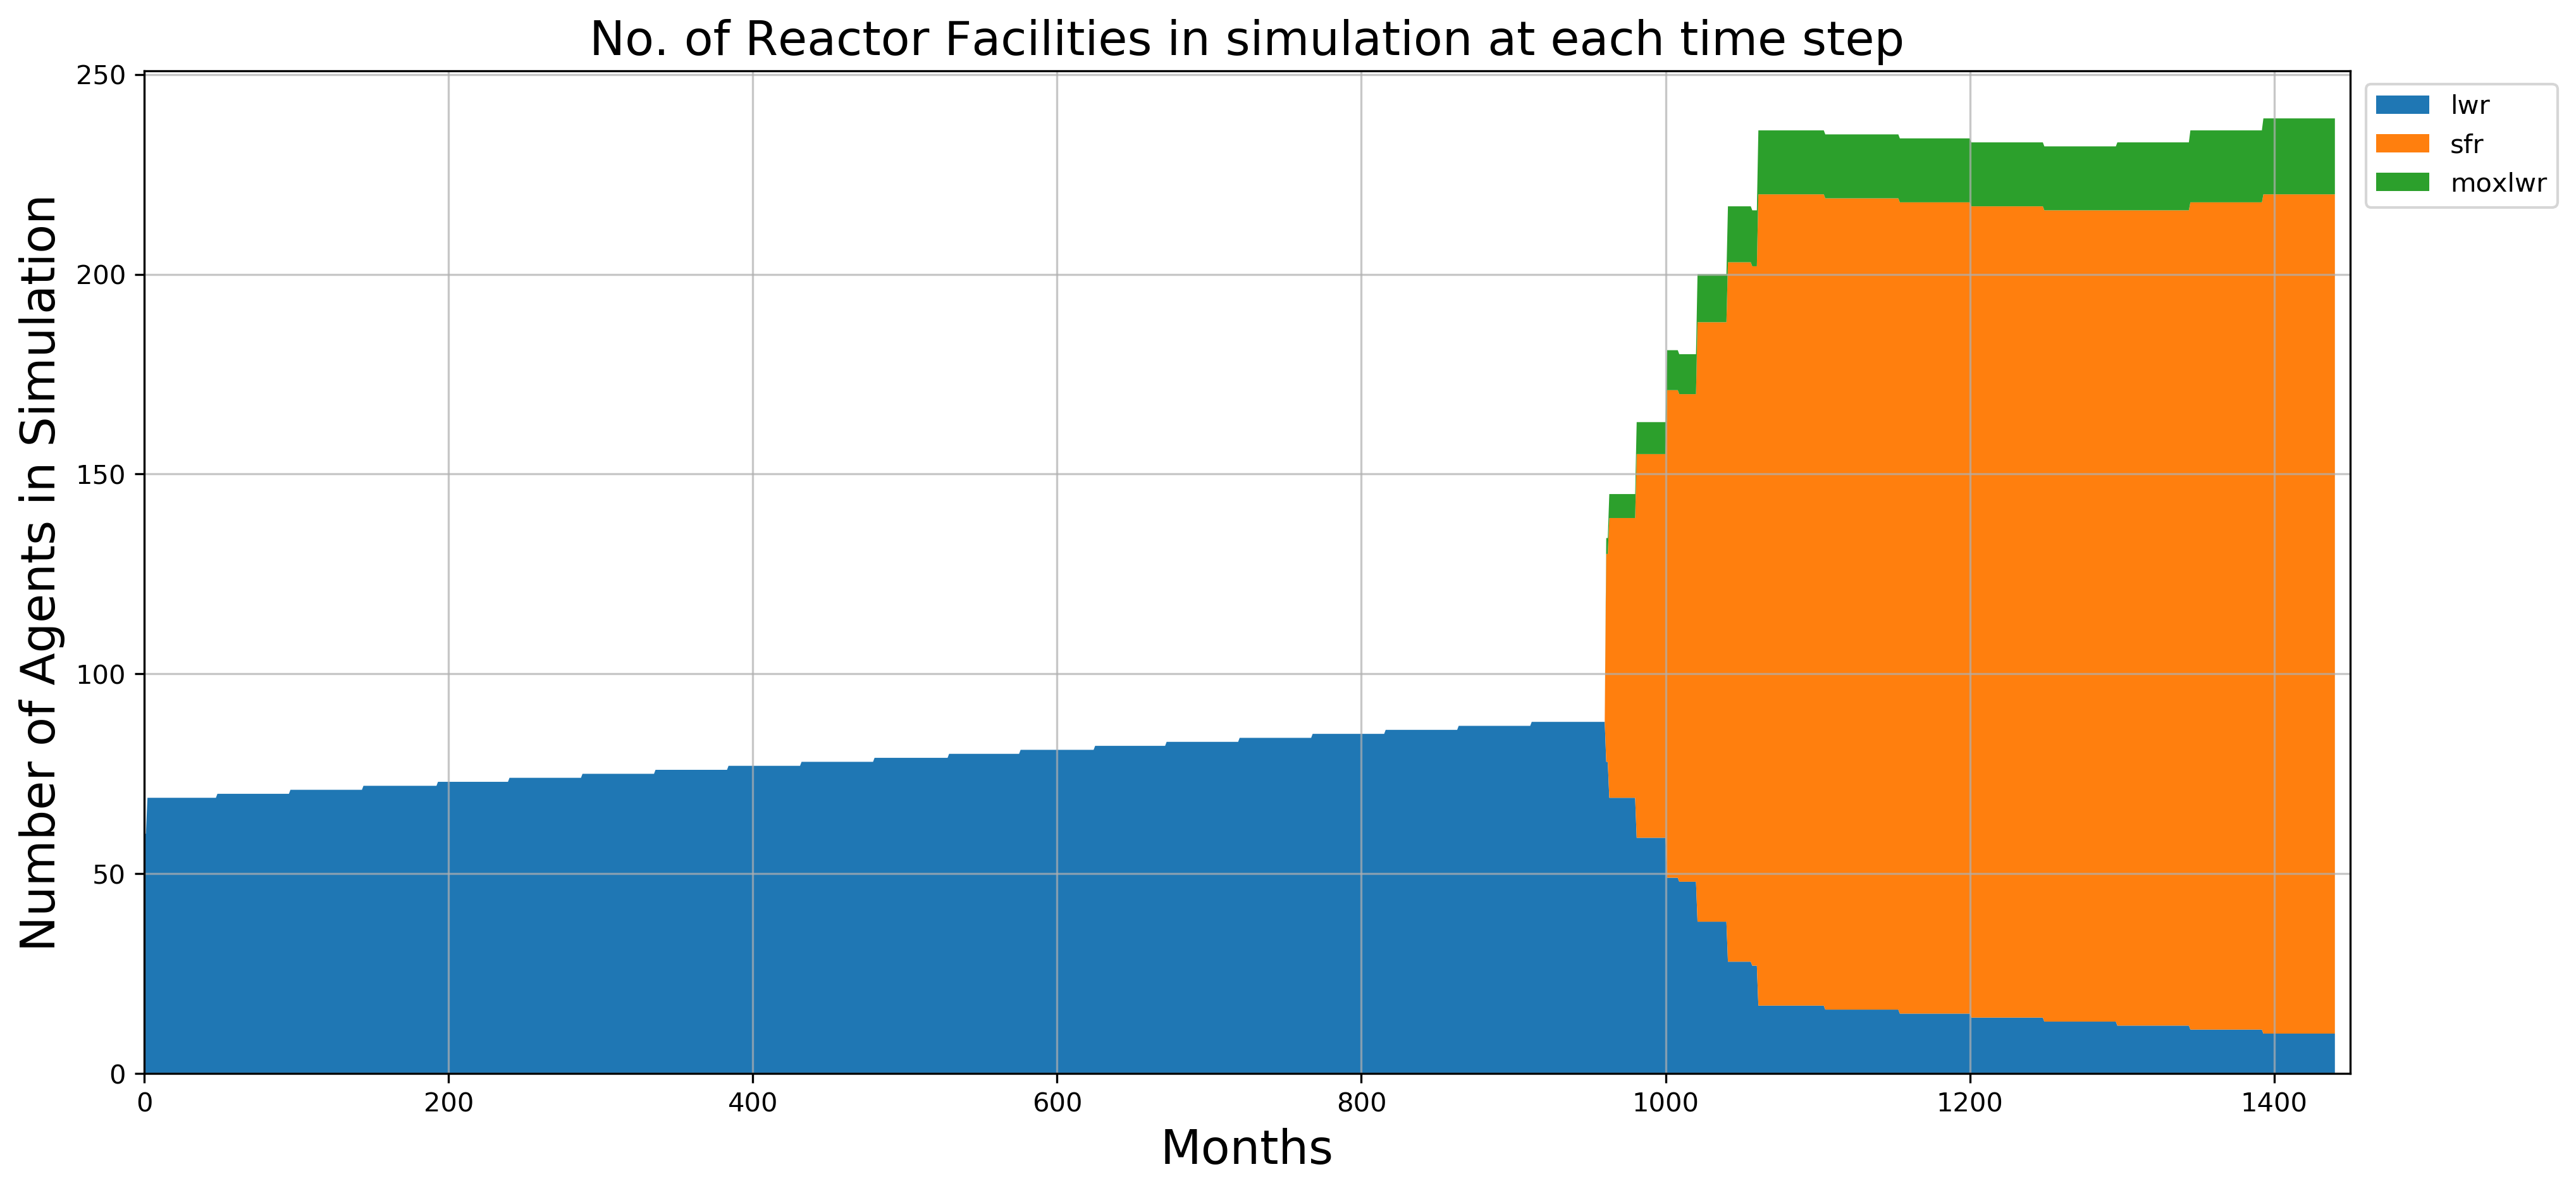
\includegraphics[width=\textwidth]{../paper/figures/eg30-stack_reactor.png}
        \end{center}
              \caption{Time dependent deployment of reactor facilities in 
              the EG01-30 linearly increasing power demand transition scenario. 
              \deploy automatically deploys reactor facilities 
              to set up a supply chain to meet constant power demand of $60000+250t/12$ MW
              during a transition from \glspl{LWR} to \glspl{SFR}}.
      \end{figure}
\end{frame}

\begin{frame}
    \frametitle{Best Performing Transition Scenarios}
    \textbf{EG01-30: Linearly Increasing Power Demand}
    \begin{figure}[htbp!]
        \begin{center}
          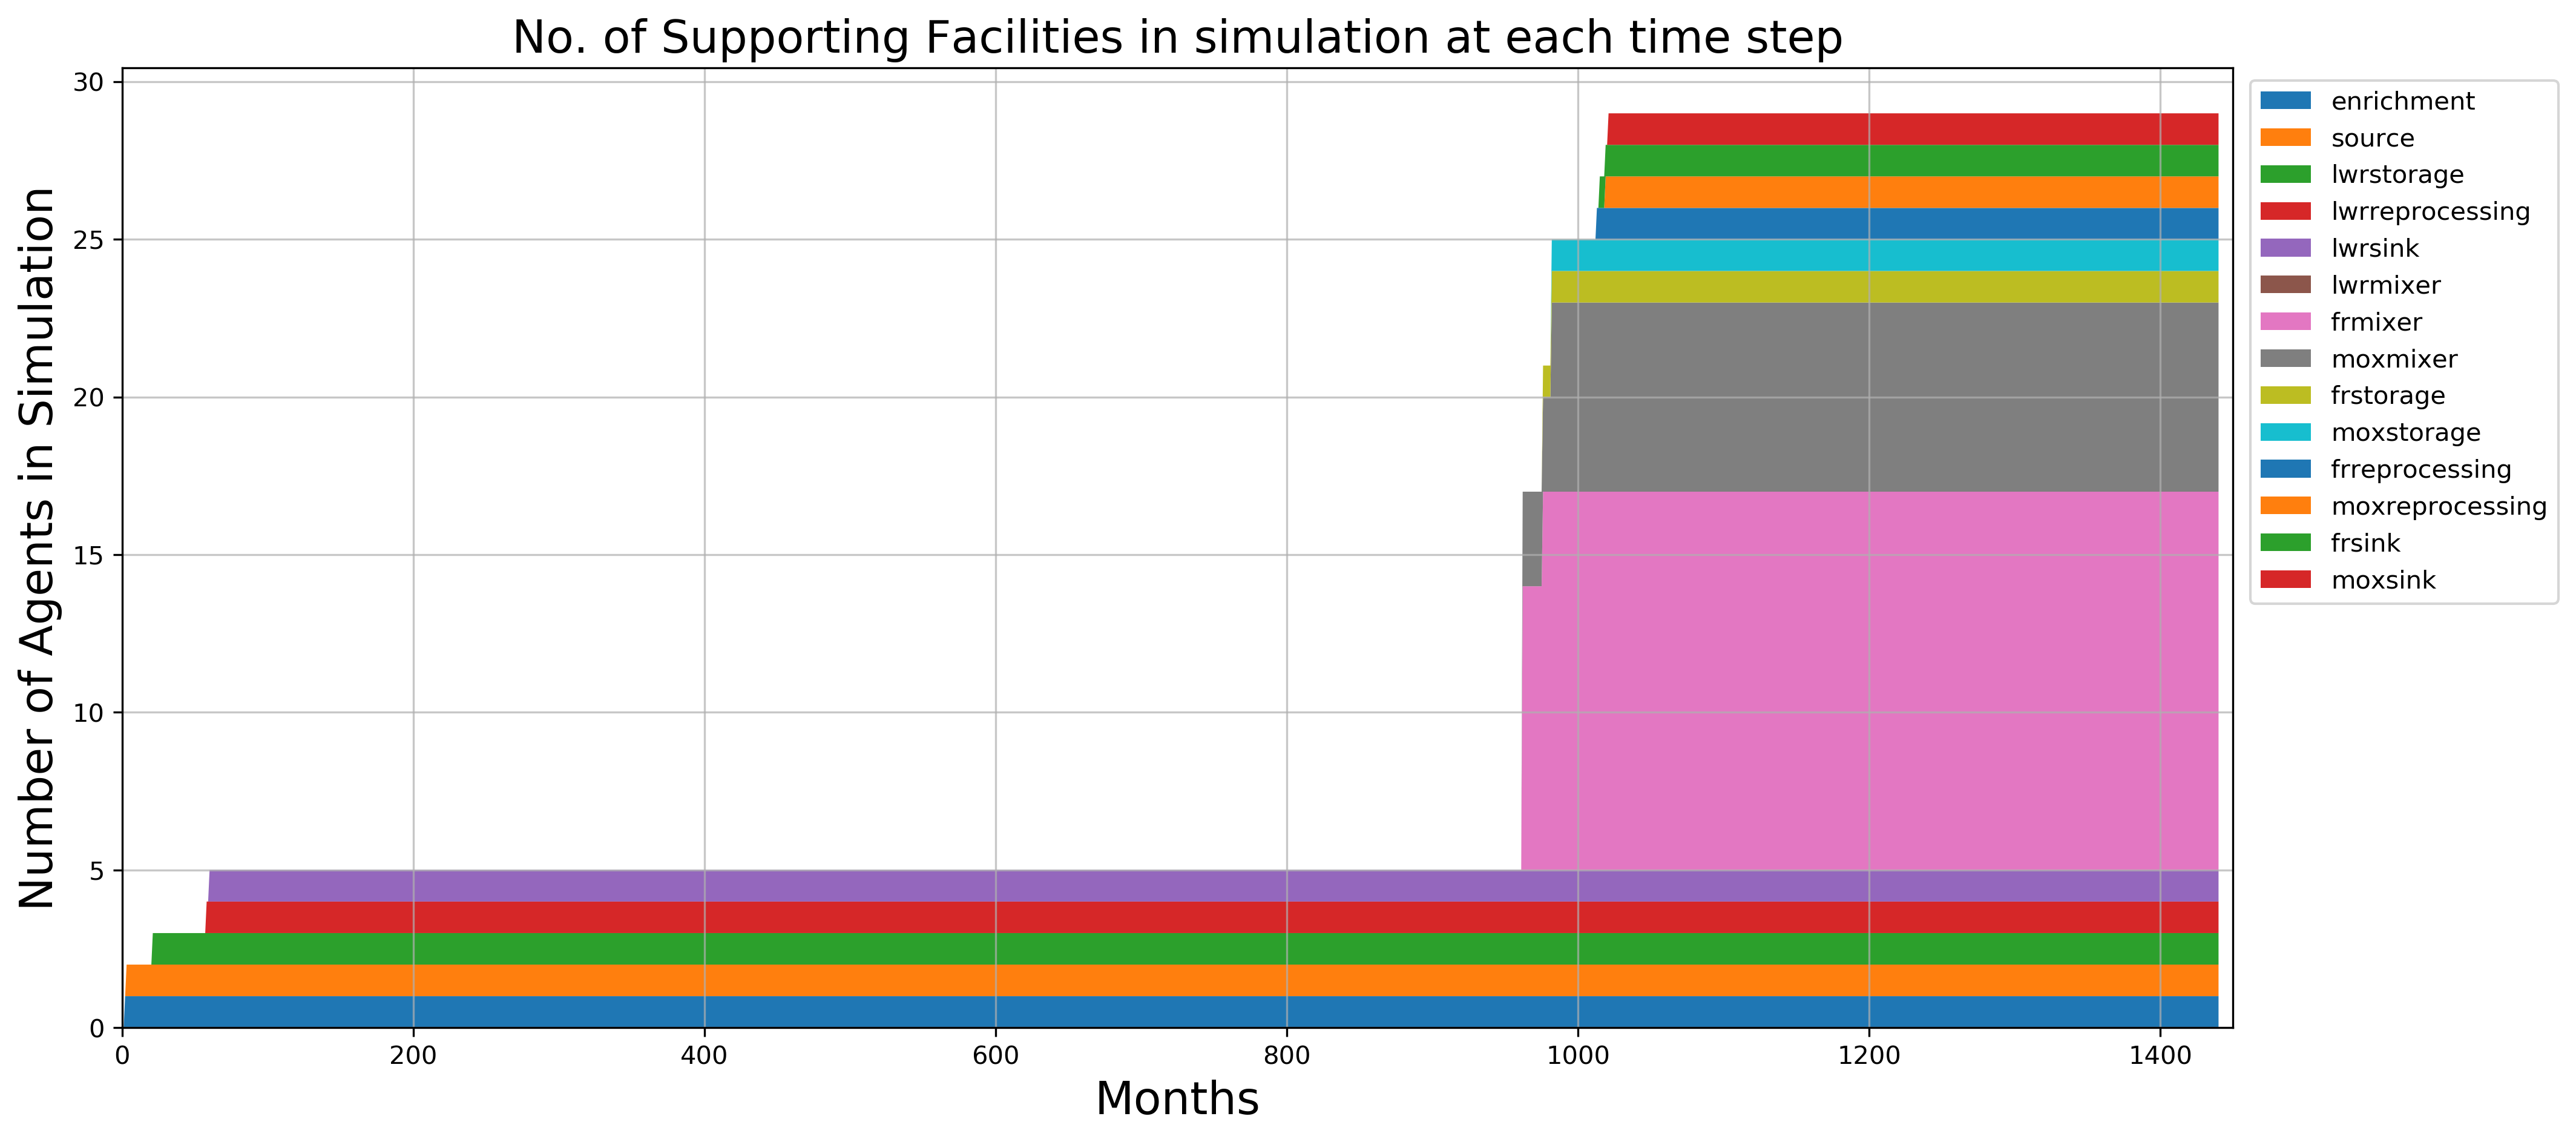
\includegraphics[width=\textwidth]{../paper/figures/eg30-stack_support.png}
        \end{center}
              \caption{Time dependent deployment of supporting facilities in 
              the EG01-30 linearly increasing power demand transition scenario. 
              \deploy automatically deploys reactor facilities 
              to set up a supply chain to meet constant power demand of $60000+250t/12$ MW
              during a transition from \glspl{LWR} to \glspl{SFR}}.
      \end{figure}
\end{frame}

\begin{frame}
    \frametitle{Best Performing Transition Scenarios}
    \textbf{Undersupply and under capacity of commodities for the best performing transition scenarios} 
    \begin{table}[]
        \centering
            \caption{Undersupply/capacity of commodities for the best performing EG01-EG23,24,29,30 transition scenarios.}
            \label{tab:all-power}
            \footnotesize
            \begin{tabularx}{\textwidth}{l|RRRR}
            \hline
            & \multicolumn{3}{|c}{\textbf{Undersupplied Time Steps}} \\ \hline
            \textbf{Transition Scenario} & EG01-EG23 & 
            EG01-EG24 & EG01-EG29 & 
            EG01-EG30 \\ 
            \textbf{Power Demand} &Constant&Linearly Increasing&Constant&Linearly Increasing \\
            \textbf{Prediction Method} &\texttt{poly}&\texttt{fft}&\texttt{poly}& \texttt{fft}\\
            \textbf{Power Supply Buffer [MW]} &0&6000&0&8000 \\ \hline
            \textbf{Commodities} \\ 
            Natural Uranium		    & 2 	& 3  &  1  & 1 \\ 
            \gls{LWR} Fuel     	    & 4 	& 6  &  1  & 2\\ 
            \gls{SFR} Fuel     	    &  0 	& 0  &  2  & 2\\ 
            \gls{MOX} \gls{LWR} Fuel &-&-&2&2 \\
            Power      				&  6 	& 7  &  4 &  5\\ 
            \gls{LWR} Spent Fuel	& 1 	& 1  & 1 & 1\\ 
            \gls{SFR} Spent Fuel     	    &  1 	& 1  &  1  & 1\\ 
            \gls{MOX} \gls{LWR} Spent Fuel &-&-&1&1 \\ \hline 
        \end{tabularx}
    \end{table}
    
\end{frame}
\section{Conclusion}
\subsection{Conclusion}
\begin{frame}
  \frametitle{Conclusion}
        These results demonstrate that by carefully selecting \deploy 
        parameters, we are able to \textbf{effectively automate deployment}
        of reactor and supporting facilities to set up 
        constant and linearly increasing power demand transition scenarios
        for EG01-23, EG01-24, EG01-29, and EG01-30 with minimal 
        power undersupply. 
        \vspace{1em}
        \\
        Not completely eliminating undersupply and under capacity of 
        commodities in the simulation is expected 
        since without time series data 
        at the beginning of the simulation, \deploy takes a few 
        time steps to collect time series data about power demand 
        to predict and start deploying reactor and supporting 
        fuel cycle facilities. 
        
\end{frame}

\subsection{Auxilliary Activities}

\begin{frame}
        \frametitle{Auxilliary Activities}

            \begin{figure}[htbp!]
        \begin{center}
          
\includegraphics[width=0.8\textwidth]{images/twofcs.png}
        \end{center}
              \caption{Technical Workshop, not funded by DOE, but well attended 
                    by DOE SA\&I community.}
      \end{figure}
\end{frame}

\begin{frame}
        \frametitle{Auxilliary Activities}


        Cyclus (particularly Wisconsin) is a key participant in the 
        Functionality Isolation Test Benchmark.
        \begin{itemize}
             \item CNRS / IN2P3 (Xavier Doligez, Marc Ernoult and Nicolas Thiollière) - CLASS
             \item University of Wisconsin - Madison (Paul Wilson and Baptiste Mouginot) - CYCLUS
             \item University of South Carolina (Robert Flanagan) - CYCLUS
             \item University of Illinois at Urbana-Champaign (Katy Huff) - CYCLUS
             \item Argonne National Lab (Bo Feng) - DYMOND
             \item Oak Ridge National Lab (Eva E. Davidson) - ORION
             \item Idaho National Lab (Ross Hays) - VISION
             \item CIEMAT (Aris Villacorta, Fransisco Alvarez) - Tr\_Evol / 
                     Evol\_code
             \item TRACTEBEL (Hubert Druenne, Bart Vermeeren) - ANICCA
             \item Univ. of technology and economics of Budapest (Mate Halasz, Màté Szieberth) - SITON
             \item Hungarian Academy of Sciences (Aron Brolly) - SITON
             \item Universidad Católica del Maule (Ivan Merino) - ANICCA
        \end{itemize}
\end{frame}

\begin{frame}
  \frametitle{Acknowledgement}
  This work is supported by U.S. Department of Energy, 
  Nuclear Energy University Program, under contract 
  \#NEUP-FY16-10512. 
  \end{frame}



%%--------------------------------%%
%%          Bibliography          %%
%%--------------------------------%%
\begin{frame}[allowframebreaks]
  \frametitle{References}
  \bibliographystyle{plain}
  {\footnotesize \bibliography{2019-09-17-anl.bib} }
\end{frame}

%%--------------------------------%%

% Examples 
% Robert: Some good examples of how to use beamer are in the example file.
% You can use this to guide the preparation of slides.


\end{document}

